% Options for packages loaded elsewhere
\PassOptionsToPackage{unicode}{hyperref}
\PassOptionsToPackage{hyphens}{url}
\PassOptionsToPackage{dvipsnames,svgnames*,x11names*}{xcolor}
%
\documentclass[
  12pt,
]{article}
\usepackage{lmodern}
\usepackage{setspace}
\usepackage{amssymb,amsmath}
\usepackage{ifxetex,ifluatex}
\ifnum 0\ifxetex 1\fi\ifluatex 1\fi=0 % if pdftex
  \usepackage[T1]{fontenc}
  \usepackage[utf8]{inputenc}
  \usepackage{textcomp} % provide euro and other symbols
\else % if luatex or xetex
  \usepackage{unicode-math}
  \defaultfontfeatures{Scale=MatchLowercase}
  \defaultfontfeatures[\rmfamily]{Ligatures=TeX,Scale=1}
  \setmainfont[]{Times New Roman}
  \setsansfont[]{Times New Roman}
\fi
% Use upquote if available, for straight quotes in verbatim environments
\IfFileExists{upquote.sty}{\usepackage{upquote}}{}
\IfFileExists{microtype.sty}{% use microtype if available
  \usepackage[]{microtype}
  \UseMicrotypeSet[protrusion]{basicmath} % disable protrusion for tt fonts
}{}
\usepackage{xcolor}
\IfFileExists{xurl.sty}{\usepackage{xurl}}{} % add URL line breaks if available
\IfFileExists{bookmark.sty}{\usepackage{bookmark}}{\usepackage{hyperref}}
\hypersetup{
  colorlinks=true,
  linkcolor=Maroon,
  filecolor=Maroon,
  citecolor=Blue,
  urlcolor=Blue,
  pdfcreator={LaTeX via pandoc}}
\urlstyle{same} % disable monospaced font for URLs
\usepackage[margin=1in]{geometry}
\usepackage{longtable,booktabs}
% Correct order of tables after \paragraph or \subparagraph
\usepackage{etoolbox}
\makeatletter
\patchcmd\longtable{\par}{\if@noskipsec\mbox{}\fi\par}{}{}
\makeatother
% Allow footnotes in longtable head/foot
\IfFileExists{footnotehyper.sty}{\usepackage{footnotehyper}}{\usepackage{footnote}}
\makesavenoteenv{longtable}
\usepackage{graphicx,grffile}
\makeatletter
\def\maxwidth{\ifdim\Gin@nat@width>\linewidth\linewidth\else\Gin@nat@width\fi}
\def\maxheight{\ifdim\Gin@nat@height>\textheight\textheight\else\Gin@nat@height\fi}
\makeatother
% Scale images if necessary, so that they will not overflow the page
% margins by default, and it is still possible to overwrite the defaults
% using explicit options in \includegraphics[width, height, ...]{}
\setkeys{Gin}{width=\maxwidth,height=\maxheight,keepaspectratio}
% Set default figure placement to htbp
\makeatletter
\def\fps@figure{htbp}
\makeatother
\setlength{\emergencystretch}{3em} % prevent overfull lines
\providecommand{\tightlist}{%
  \setlength{\itemsep}{0pt}\setlength{\parskip}{0pt}}
\setcounter{secnumdepth}{-\maxdimen} % remove section numbering
\usepackage{longtable}
\usepackage{threeparttable}
\usepackage{rotating}
\usepackage{booktabs}
\usepackage{longtable}
\usepackage{array}
\usepackage{multirow}
\usepackage{wrapfig}
\usepackage{float}
\usepackage{colortbl}
\usepackage{pdflscape}
\usepackage{tabu}
\usepackage{threeparttable}
\usepackage{threeparttablex}
\usepackage[normalem]{ulem}
\usepackage{makecell}
\usepackage{xcolor}

\title{\vspace{1cm}Collective Speech Among Addiction Treatment Organizations\\
~\\}
\author{Gabriel Varela\\
Duke University}
\date{April 28th, 2021\\
~\\}

\begin{document}
\maketitle
\begin{abstract}
\noindent\setstretch{1}Scholars have shown that speech varies across for-profit, non-profit, and public organizations. Yet none have explored the possibility that the relationship between speech and ownership varies across ownership type. I investigate this possibility in the market for addiction treatment, in which a recent influx of for-profit addiction treatment services has been met with skepticism and reports of patient abuse. By examining the online speech of every addiction treatment service in New York State, I highlight the extent to which the market is experiencing or resisting isomorphic change by measuring collective and distinctive language among for-profit, non-profit and public organizations. I find that while for-profit and public organizations exhibit some collective speech, non-profits do not. Auxiliary analysis also reveal that for-profit organizations use different repertoires of language when describing patients and clients. Overall, results suggests that language coheres differently, or fails to cohere, given ownership type. \vspace{.8cm}
\end{abstract}

\setstretch{2}
\clearpage

\hypertarget{introduction}{%
\section{Introduction}\label{introduction}}

How do new entrants to an organizational field seek legitimacy? The ability to communicate with clients is, particularly in a healthcare market, fundamental to organizational success (Bail \protect\hyperlink{ref-bail2016}{2016}). Organizations may look to their peers as models for how to speak, and in turn signal legitimacy by leveraging specific repertoires of speech. In this article, I draw from the literature in organizational sociology, moral markets, medicalization and the growing field of computational methods to better understand the factors influencing organizational speech in addiction treatment facilities in New York State. In particular, I consider two competing sets of organizational theories to explore how new entrants seeking legitimacy construct a common narrative. On the one hand, isomorphism (DiMaggio and Powell \protect\hyperlink{ref-dimaggio1983}{1983}) predicts that new entrants should begin to resemble established organizations in the field as a reaction to normative pressure. If an isomorphic process is in fact taking place, then we should expect organizations to speak similarly and not observe clustering. On the other hand, contemporary criticisms of the isomorphic approach have asked scholars to consider the way morality becomes infused into markets and leads certain organizations to resist isomorphic change. These moral market approaches predict that new entrants should react to pressure by creating a unique and distinctive blend of market and treatment values that justify their practice (Fourcade and Healy \protect\hyperlink{ref-fourcade2007}{2007}; Reich \protect\hyperlink{ref-reich2014}{2014}). In this view, the field of addiction treatment should feature strong speech clusters.

\vspace{12pt}

Scholars have been particularly interested in the ways in which organizational speech clusters around shared ownership type---being a for-profit, non-profit or public organization. Indeed, two organizations of the same ownership type often share key characteristics such as income streams, tax regulations and legal statuses. As a result, there is evidence that organizational speech and culture varies both across and within ownership type (DiMaggio and Anheier \protect\hyperlink{ref-dimaggio1990}{1990}; Mohr \protect\hyperlink{ref-mohr1994}{1994}; Erreygers and Jacobs \protect\hyperlink{ref-erreygers2005}{2005}; Weber and Dacin \protect\hyperlink{ref-weber2011}{2011}; Paxton, Velasco, and Ressler \protect\hyperlink{ref-paxton2020}{2020}; Zhao and Oh \protect\hyperlink{ref-zhao2021}{2021}). But not all ownership types are viewed equally within and outside of the field. Particularly in a highly moralized healthcare market such as addiction treatment, some ownership types are viewed as more legitimate, while others experience strong normative pressure to prove their legitimacy. And yet, little research has studied how organizational speech coheres at the field level in the face of this differentially-distributed normative pressure.

\vspace{12pt}

Illuminating this process would inform both organizational and health scholarship. Currently, research on organizations across sub-disciplines largely considers ownership types as de facto coherent categories. Few studies have looked at speech across ownership types in a given field (Fuchs \protect\hyperlink{ref-fuchs2005}{2005}; Wetts \protect\hyperlink{ref-wetts2020}{2020}), and those who do implicitly assume that finding difference in speech across ownership types is equivalent to within-ownership similarity of speech. In other words, evidence of inter-ownership speech difference yield assumptions of intra-ownership similarity. Although perhaps true in some cases, this de-emphasizes the possibility that the relationship between ownership and speech---not just speech itself---may be significantly different across ownership types. Some ownership types may be associated with more coherence--and leverage more repertoires to build that coherence--than others. In a healthcare market, such coherence (or lack thereof) may quickly translate to differential access to a particular quality of care.

\vspace{12pt}

Health scholars have noted the importance of for-profit ownership on quality of care in the addiction field (Bachhuber, Southern, and Cunningham \protect\hyperlink{ref-bachhuber2014}{2014}; Beetham et al. \protect\hyperlink{ref-beetham2021}{2021}). Key regulatory changes in the United States have made treatment more accessible than ever, coinciding with repeated waves of opioid epidemics(Rudd \protect\hyperlink{ref-rudd2014}{2014})(Center for Disease Control 2020). These changes have resulted in significant transformations in the market, with for-profits representing 29\% of the field in 2009 to 40\% in 2019 (Substance Abuse and Mental Health Services Administration 2020). Profit-seeking motive in the provision of addiction care is often seen as a root cause of the problem, particularly in the wider public (Segal \protect\hyperlink{ref-segal2017}{2017}). As a result, for-profit organizations are under a particular normative pressure to legitimize their approach. Yet, policy scholars note that language remains a powerful tool of for-profit organizations when recruiting patients, which is not the case for other ownership types (Beetham et al. \protect\hyperlink{ref-beetham2021}{2021}). Deploying social theory to understand the contours of the field can begin to answer the puzzle described by policy scholarship.

\vspace{12pt}

I investigate the online speech of every certified addiction treatment organization in New York State in 2020. I hypothesize that for-profit organizations pull from a shared pool of language in order to legitimate the for-profit approach, and that they also pull from multiple repertoires of speech. Conversely, I hypothesize that non-profit and public organizations---who do not experience comparable pressure---will exhibit less collective speech. Until recently, social scientists lacked the ability to analyze organizational speech at scale. Most of the work published in the area of addiction treatment uses qualitative methods (Iacobucci and Frieh \protect\hyperlink{ref-iacobucci2018}{2018}), although computational approaches are being deployed in other areas of organizational research (Paxton et al. \protect\hyperlink{ref-paxton2020}{2020}; Wetts \protect\hyperlink{ref-wetts2020}{2020}; Haber \protect\hyperlink{ref-haber2021}{2021}). In this article, I use computational text-analysis techniques to systematically measure collective speech by ownership type among addiction treatment organizations. In addition, I do so net of several material factors that we might expect lead to similar speech, such as geographic closeness. The use of computational approaches iteratively with a close reading of documents is an increasingly popular approach (Nelson \protect\hyperlink{ref-nelson2017}{2017}) that can complement existing scholarship.

\hypertarget{the-history-of-addiction-treatment}{%
\section{The History of Addiction Treatment}\label{the-history-of-addiction-treatment}}

Until 1939, historical efforts to handle addiction have been limited. Most individuals suffering from substance abuse were housed in hospitals and almshouses and rarely received necessary treatment. Those few who undertook treatment were usually a responsibility of the state. Despite early attempts to realize treatment---mentions of sober houses can be found as early as 1783---the first effective contemporary endeavors came in 1939 with the founding of Alcoholics Anonymous. At that point hospitals had grudgingly treated alcoholics and considered them difficult patients who failed to pay their bills. A key part of AA's success was changing the framing of addiction from a moral weakness to a medical illness (Henninger and Sung \protect\hyperlink{ref-henninger2014}{2014}). Following this landmark change, grass roots non-profits like Pioneer House and Hazelden Farm effectively refocused medical attention on substance use disorder (SUD) and started to change public perceptions on the issue. The field of substance abuse became largely driven by non-profit organizations with a dual focus on local community issues (particularly in major cities like New York and San Francisco) and an interest in changing national public perceptions. It is these same players who shaped contemporary treatment approaches through a combination of inpatient detoxification, medical treatment and outpatient follow-up work.

\vspace{12pt}

While for-profit organizations were far from absent during this period spanning the second half of the 20th century, they took a back seat both numerically and politically. A key issue for profit-seeking organizations is accessing a wide enough pool of patients. A part of the clientele is willing and able to pay out of pocket for substance abuse treatment: those clients were and still are at the core of the for-profit substance abuse treatment field, exemplified by the luxury rehab compound. However, the larger portion of individuals who pay for treatment through public and private insurance remained out of reach, with most plans failing to provide coverage for SUD treatment in any form. This changed with the 2008 Mental Health Parity and Addiction Equity (MHPAE) Act which enforced insurance parity between substance abuse treatment and other medical needs, opening treatment opportunities for millions of individuals in need of care (Barry, Huskamp, and Goldman \protect\hyperlink{ref-barry2010}{2010}). This effect was further compounded in 2010 by the Affordable Care Act (ACA) which extended insurance coverage---at states' discretion---to thousands more (Abraham et al. \protect\hyperlink{ref-abraham2017}{2017}; Maclean and Saloner \protect\hyperlink{ref-maclean2019}{2019}). These two regulatory changes, combined with a second wave of the opioid epidemic (Rudd \protect\hyperlink{ref-rudd2014}{2014}) created the conditions for a major expansion of the for-profit market: in 2009---a year after the passing of the MHPAE act---for profit substance abuse treatment represented 29\% of the national field. In 2019, for-profit ownership makes up 40\% of all organizations in the field. Spending has changed accordingly, with private (as opposed to public) recipient organizations increasing their share of total SUD spending from 31\% in 2006 to 43\% in 2015 (Substance Abuse and Mental Health Services Administration 2015).

\begin{figure}
\centering
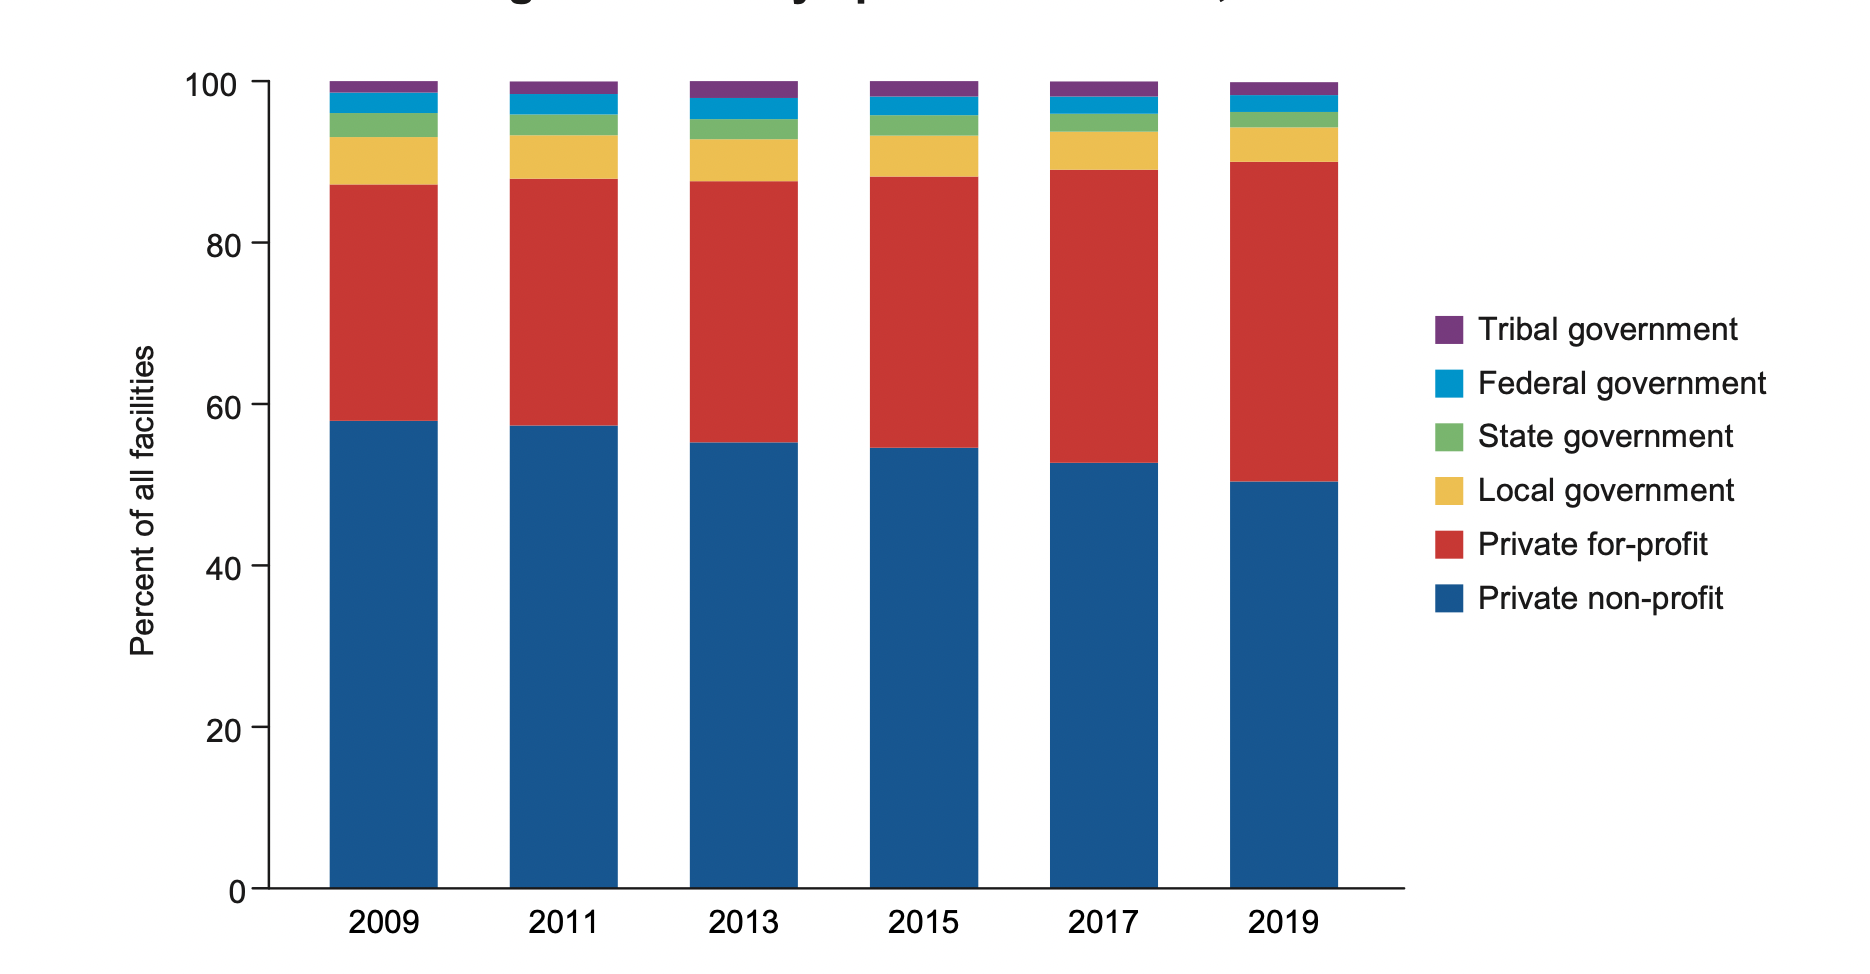
\includegraphics{/Users/gabe/Documents/Classes/Second year paper Repro/Collective-Speech-Among-Addiction-Treatment-Organizations/figures and tables/stacked_barchart.png}
\caption{\label{fig:unnamed-chunk-2}\textit{Facility operation - Percent, 2009-2019 (Source: N-SSATS 2019)}}
\end{figure}

While the previous luxury for-profit program remains an important actor in field of substance abuse, new for-profit services have emerged to answer regulatory changes and demand. What is described as a veritable ``gold rush'' in the market for addiction (Mann \protect\hyperlink{ref-mann2021}{2021}) did not, however, only bring in good actors. A slew of anecdotal evidence has shed light on the potential for heterogenous quality of care (Meyer \protect\hyperlink{ref-meyer2018}{2018}), and even cases of outright fraud, as in the case in the market for urinary testing (Segal \protect\hyperlink{ref-segal2017}{2017}). Beetham et al. (\protect\hyperlink{ref-beetham2021}{2021}) performed an audit study of for-profit ``detox'' programs, finding that they may charge up to twice as much as comparable non-profit services---while simultaneously utilizing aggressive recruitment techniques. The National Association of Addiction Treatment Providers (NAATP) themselves have recognized this as a field-wide crisis and centered ethics as a core part of their most recent strategic plan, going so far as to begin ``the unusual undertaking of removing numerous members of the association at considerable financial loss and strictly evaluating ongoing membership for ethical compliance'' {[}emphasis added{]} (National Association of Addiction Treatment Providers 2019).

\vspace{12pt}

To capture the attention of a population that is either insured for treatment or that can afford treatment out of pocket, for-profit organizations must leverage a strategic identity---a cultural presentation of self that is projected toward clients and families. In addition, they must do so while facing strong normative pressures from both within and outside the field. Studying these new actors in an increasingly moralized field is an opportunity to ask: with their legitimacy threatened, do for-profit organizations cohere around common speech more than other ownership types? If so, do they imitate more established---and better regarded---non-profits? Or instead, do they attempt to speak distinctively and legitimate their approach?

\hypertarget{mechanisms-shaping-coherence-by-ownership}{%
\section{Mechanisms Shaping Coherence by Ownership}\label{mechanisms-shaping-coherence-by-ownership}}

\hypertarget{isomorphism}{%
\subsection{\texorpdfstring{\emph{Isomorphism}}{Isomorphism}}\label{isomorphism}}

Faced with the threat of losing all legitimacy, one approach for new for-profit addiction treatment organizations may be to imitate established non-profit actors. This is precisely what institutional theories expect is taking place within a given market. DiMaggio and Powell (\protect\hyperlink{ref-dimaggio1983}{1983}) argue that new entrants to a market experience various forms of pressures, including normative pressures, particularly under conditions of uncertainty. These pressures lead to a process of isomorphism---a homogenization of organizational structures. The authors provide several hypotheses about the predictors of isomorphic change, including a reliance on credentialing, transactions with state agencies, few alternative organizational models and uncertain technological change.

\vspace{12pt}

All four of these predictors are highly salient in the field of addiction treatment. For instance, addiction treatment organizations can undergo several instances of credentialling at the professional level (NAATP), the state level (OASAS) and the federal level (SAMHSA). The Medicaid reimbursements that form an increasingly important part of income streams represent a systematic transaction with state agencies. As noted previously, few treatment alternatives exist, and the few existing ones are further restricted by strict medical guidelines (American Society of Addiction Medicine 2015). Lastly, addiction medicine is an evolving technological field, as is exemplified by the rapid successive releases of methadone, buprenorphine and naltrexone, all with distinct implications for care.

\vspace{12pt}

Isomorphism was further adapted to the healthcare field by Scott et al. (\protect\hyperlink{ref-scott2000}{2000}) and applied to particular healthcare systems to study how fields are changing (or not) (Clarke and Estes \protect\hyperlink{ref-clarke1992}{1992}; Macfarlane et al. \protect\hyperlink{ref-macfarlane2013}{2013}). For example, Hughes and Vincent-Jones (\protect\hyperlink{ref-hughes2008}{2008}) explore the changing configuration of a modernized British NHS, finding relative influences of each type of isomorphic pressure. Institutional theory has also made its way to the specific study of addiction care, where researchers have found evidence of the isomorphic process in adaptation to culturally responsive care (Guerrero and Kim \protect\hyperlink{ref-guerrero2013}{2013}; Guerrero et al. \protect\hyperlink{ref-guerrero2016}{2016}) and expect continued homogenization leading to firm consolidation (Corredoira and Kimberly \protect\hyperlink{ref-corredoira2006}{2006}). A growing body of empirical research suggests that funding and regulation have made services increasingly responsive to client needs in general (Simpson, Joe, and Rowan-Szal \protect\hyperlink{ref-simpson2007}{2007}) and in the criminal justice system in particular (Chavez \protect\hyperlink{ref-chavez2012}{2012}). Staton, Andraka-Christou, and Watson (\protect\hyperlink{ref-staton2021}{2021}) describe the isomorphic process in a jail diversion program that is changing its focus toward persons with opioid use disorder.

\vspace{12pt}

The isomorphic lens plays an important role in the ways that addiction researchers have approached change in the addiction treatment field. Since ownership type structures many of the characteristics that might foster or impede isomorphic change, studies naturally rely on comparisons across these types to determine how isomorphic the field has become. The overwhelming majority of studies focus on organizational structure, funding and activity as evidence for isomorphic change. Much less is known about organizational speech. Scholars have focused on single organizations (Jordan \protect\hyperlink{ref-jordan2015}{2015}) or comparisons between two categories such as public and private (Iacobucci and Frieh \protect\hyperlink{ref-iacobucci2018}{2018}). Zhao and Oh (\protect\hyperlink{ref-zhao2021}{2021}) test whether shared ownership is predictive of shared framing around the opioid epidemic, although their analysis focuses on regulatory agencies and pharmaceutical corporations rather than treatment providers.

\vspace{12pt}

According to institutionalist explanations of form emergence, recent for-profit entrants to the addiction treatment market should arrange their structure, treatments and behaviors with clients in function of what is perceived as good and appropriate. The same could be expected of speech. In a market where for-profits are seeking to present themselves as a legitimate course of action for treatment, they may look to established actors for frames and vocabulary. A visualization of the discursive field of addiction treatment may look like scenario A in Figure 2---an ideal-typical scenario in which the addiction field has niches based on expertise, but where ownership type plays no clear role in clustering.

\hypertarget{moral-markets}{%
\subsection{\texorpdfstring{\emph{Moral Markets}}{Moral Markets}}\label{moral-markets}}

Growing from this seminal research stream on isomorphism, a group of scholars have sought to explain deviations from the simple isomorphic process. For example, Reich (\protect\hyperlink{ref-reich2014}{2014}) explores why three non-profit hospitals in the same area of Northern California exhibit qualitatively different behavior, framing of care and structure despite facing the conditions for isomorphism---including shared ownership type. He draws from Stinchcombe (\protect\hyperlink{ref-stinchcombe2000}{2000}) to argue that moral missions become ``imprinted'' (Reich \protect\hyperlink{ref-reich2014}{2014}:1579) in the organization, which allows them to resist mimetic pressures. In Reich's case, non-profit ownership is not a coherent category of hospitals; founding year is a much more useful categorization. This focus on the moral and social components of markets asks us to read organizations as having moral projects, from which moralized markets may emerge (Fourcade and Healy \protect\hyperlink{ref-fourcade2007}{2007}).

\vspace{12pt}

Not all moral markets exhibit differentiation within ownership type. In fact, the moralization of a market can translate into normative pressures which undergird the isomorphic process. Both the commodification of motherhood (Turco \protect\hyperlink{ref-turco2012}{2012}) and scarcity in hospice care (Livne \protect\hyperlink{ref-livne2014}{2014}) are forces which exert similar pressure on the whole field. However, adding complexity to the forces that shape imitation between organizations allows for the possibility of markets to remain heterogenous. Additional evidence of this has been found in the trade of blood and organs (Healy \protect\hyperlink{ref-healy2010}{2010}), mutual funds (Lounsbury \protect\hyperlink{ref-lounsbury2007}{2007}), manufacturing (Greenwood et al. \protect\hyperlink{ref-greenwood2010}{2010}) and cadavers (Anteby \protect\hyperlink{ref-anteby2010}{2010}). Although ownership type isn't always the primary focus, these scholars often reveal how different market orientations can help organizations resist isomorphic forces.

\vspace{12pt}

While the addiction treatment field exhibits the conditions necessary for isomorphism across ownership types, it also presents similar features to moralized markets. This is particularly the case when publics find for-profit interests to be dissonant with the provision of care (You et al. \protect\hyperlink{ref-you2016}{2016}). The worry about whether an organization is in the field for ``the right reasons'' is present in the field of substance abuse treatment as well (Storbjörk and Stenius \protect\hyperlink{ref-storbjork2019}{2019}; Beetham et al. \protect\hyperlink{ref-beetham2021}{2021}). If the disproportionate normative pressure experienced by for-profit addiction treatment organizations stems from doubts about their moral orientation, we may expect that these actors recognize themselves as a collective under threat and cluster together to legitimate the for-profit approach--leading to several different clusters of speech at the field level. This possibility is presented as scenario B in Figure 2. As such, I hypothesize that:

\vspace{12pt}

\textbf{Hypothesis 1:} Sharing for-profit ownership will be predictive of discursive similarity.

\vspace{12pt}

On the other hand, non-profit and public organizations don't tend to receive the same scrutiny over their moral orientation. In fact, I have shown that non-profit actors are the heroes of the addiction treatment story. Untainted by profit-seeking motives, their approach is considered more patient-centered. In addition, non-profit and public organizations tend to work with patients who have more complex comorbidities such as homelessness and other mental health issues (Beetham et al. \protect\hyperlink{ref-beetham2021}{2021}). I argue that non-profits and public organizations are not viewed as a collective defined by their ownership, but rather as individual organizations embedded in their local communities. As a result, I hypothesize that:

\vspace{12pt}

\textbf{Hypothesis 2:} Sharing non-profit and public ownership will be less predictive of discursive similarity than sharing for-profit ownership.

\begin{figure}
\centering
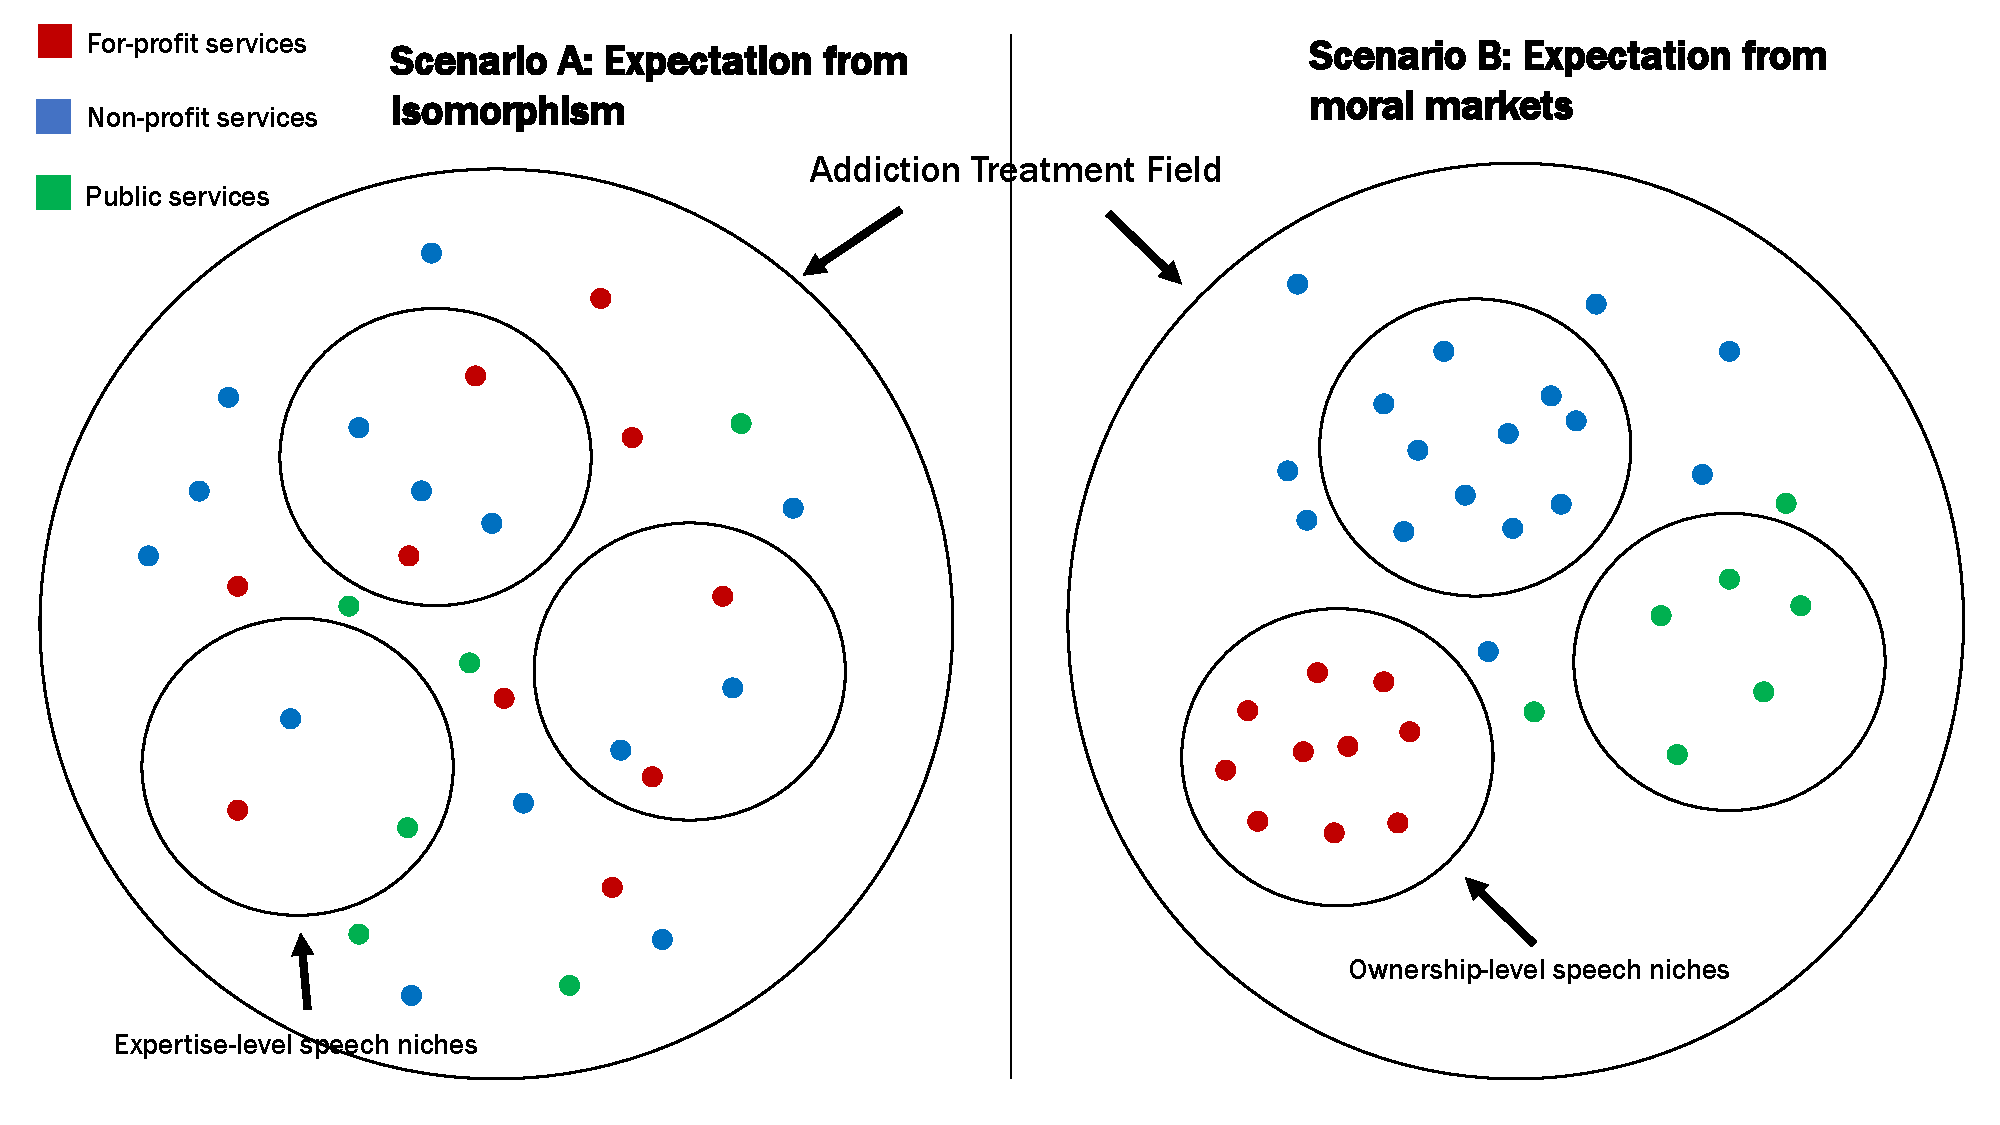
\includegraphics{/Users/gabe/Documents/Classes/Second year paper Repro/Collective-Speech-Among-Addiction-Treatment-Organizations/figures and tables/scenarios.pdf}
\caption{\label{fig:unnamed-chunk-3}\textit{Expectations for the addiction field}}
\end{figure}

\hypertarget{content-of-collective-speech}{%
\subsection{\texorpdfstring{\emph{Content of collective speech}}{Content of collective speech}}\label{content-of-collective-speech}}

If my hypothesis is correct and certain ownership types cohere more than others, the natural next question to ask is what that speech consists of. Instead of looking at all words, I focus on a particular object being spoken about, namely the patients and clients themselves. This has two main benefits over a more exhaustive analysis: first, references to patient and client are often parts of the websites that are referring to the reader directly, enabling me to focus on sections of the text where organizations make their most direct appeals. Second, it allows me to analyze the words using existing concepts formulated by medical sociologists. Unsurprisingly, a main focus of medical sociologists has been the patient, seeking to understand how the ``sick role'' (Parsons \protect\hyperlink{ref-parsons1951}{1951}) is constructed by institutional forces. The movement from the political sphere to the medical sphere---otherwise known as medicalisation (Conrad \protect\hyperlink{ref-conrad1992}{1992})---has been key to understanding how the definition of addicted patient has developed across racial, gender and age lines (Acker \protect\hyperlink{ref-acker2002}{2002}; Conrad and Schneider \protect\hyperlink{ref-conrad2010}{2010}; Granfield and Reinarman \protect\hyperlink{ref-granfield2014}{2014}). Discourse studies have systematically been leveraged to operationalize definitions of addicted patienthood (Andersen \protect\hyperlink{ref-andersen2015}{2015}; Selbekk and Sagvaag \protect\hyperlink{ref-selbekk2016}{2016}; Hatcher, Mendoza, and Hansen \protect\hyperlink{ref-hatcher2018}{2018}; Riboni \protect\hyperlink{ref-riboni2020}{2020}).

\vspace{12pt}

However, research in this tradition has either focused on a particular ownership setting, such as public methadone clinics (Bourgois \protect\hyperlink{ref-bourgois2000}{2000}), or compared across ownership type (Iacobucci and Frieh \protect\hyperlink{ref-iacobucci2018}{2018}). Iacobucci and Frieh (\protect\hyperlink{ref-iacobucci2018}{2018}) compare the websites of 20 public organizations and 20 private addiction treatment organizations in New York State and find more controlling language in public offerings. They focus their analysis on a priori coding schemes (criminality, holism etc.,) and do not distinguish between for-profit and non-profit private organizations. These approaches have the benefit of capturing how particular organizations structure and contest the terrain of addiction. They are not as effective at systematically revealing similarity in language between and within ownership types. Building off their work, I propose to leverage computational methods to explore the variety of repertoires used by organizations of a given ownership type when defining patient and client. Because public organizations are largely defined by their connection with the state, I expect that these organizations will be using simple formal language reminiscent of large bureaucracies. Additionally, public services are often located in hospitals and consequently receive patients regardless of their ability to be attractive.

\vspace{12pt}

\textbf{Hypothesis 3:} Public organizations will use a single repertoire when speaking of ``patient'' and ``client''

\vspace{12pt}

Conversely, I hypothesize that for-profit and non-profit organizations need to engage readers in several different ways in order to be competitive. Marketing services effectively on their websites means acknowledging patient's uncertainty about treatment, fear of disclosure and questions about amenities, to name just a few.
For example, I expect that for-profit organizations will present themselves as competent actors that have two advantages over the other ownership types: the efficiency of markets and a more holistic approach to care. I expect that non-profit organizations will discuss their seniority in the field and a focus on community. This leads me to my last hypothesis:

\vspace{12pt}

\textbf{Hypothesis 4:} For-profit and non-profit organizations will use several repertoires when speaking of ``patient'' and ``client''

\vspace{12pt}

\hypertarget{websites-as-sites-of-organizational-speech}{%
\subsection{\texorpdfstring{\emph{Websites as sites of organizational speech}}{Websites as sites of organizational speech}}\label{websites-as-sites-of-organizational-speech}}

The study of mission statements as organizations' moral orientation is ubiquitous in organizational research. Paxton et al. (\protect\hyperlink{ref-paxton2020}{2020}) shows how displaying emotion in non-profit mission statements leads to increased donations and volunteership, while Bail (\protect\hyperlink{ref-bail2016}{2016}) reveals how striking the right balance in number of topics allows for more engagement. Because online text data is an opportunity to see culture \emph{in situ} (Bail \protect\hyperlink{ref-bail2014}{2014}), researchers have observed semantic divisions among actors in various markets including climate change (Wetts \protect\hyperlink{ref-wetts2020}{2020}) and education (Haber \protect\hyperlink{ref-haber2021}{2021}). Haber (\protect\hyperlink{ref-haber2021}{2021}) finds that charter schools, as relatively new entrants to the educational market, leverage a common set of discursive symbols on their website that attract a particular clientele. The understanding of markets as discursive fields (Mohr and Duquenne \protect\hyperlink{ref-mohr1997}{1997}) is attractive to researchers because it gets us closer to the cultural orientations of organizations. In step with this research, I use organizational websites to draw out the similarities, or lack thereof, between addiction treatment organizations of varying ownership types.

\hypertarget{data-and-methods}{%
\section{Data and Methods}\label{data-and-methods}}

\hypertarget{data}{%
\subsection{\texorpdfstring{\emph{Data}}{Data}}\label{data}}

Addiction treatment organization websites appeal to potential clients and families: the type of care they provide, how they view the client and the expertise of their practitioners. Undoubtedly, some website visitors do not take for granted what they read in mission statements. This is particularly true when corresponding treatment aggregators (eg., \url{https://startyourrecovery.org}, \url{https://www.recovery.org}) often appear among top searches. Because I am analyzing self-descriptions from websites, it is less likely that the information presentation is affecting user choice. However, this should have no bearing on organization's use of information as a way to promote a unique collective identity toward the field as a whole.

\vspace{12pt}

I use the National Survey of Substance Abuse Treatment Services (N-SSATS) provided by the Substance Abuse and Mental Health Services Administration (SAMHSA) to identify addiction treatment services in New York State. SAMHSA reports a response rate of 91\% overall, and 95.1\% in New York State. In the United-States, considerable differences in state legislation---namely around insurance coverage---means two sets of organizations in different states may be operating under different market constraints. I limit my analysis to New York State to ensure that all the observed organizations are comparable. Future research could systematically identify state difference in addiction treatment (Grogan et al. \protect\hyperlink{ref-grogan2020}{2020}) and extend this research to capture regional difference. Additionally, New York is a useful example state: it houses a large number of organizations and varied rural and urban settings.

\vspace{12pt}

At the time of writing, SAMHSA identified 854 services as providing substance abuse treatment in New York State. N-SSATS provides an organization website for each surveyed service---if none are provided, I researched the organization myself using the service name and location. I was able to identify 740 services in total. I could not confidently associate a website with the remaining 114 services, so I dropped them out of the dataset. 547 services are non-profit, 126 are for-profit and 67 are public. Several services (observations in the N-SSATS) may be managed by the same organization and presented on the same website. I find 268 unique organizations and websites.

\hypertarget{dependent-variable}{%
\subsection{\texorpdfstring{\emph{Dependent Variable}}{Dependent Variable}}\label{dependent-variable}}

For each of the 268 organizations, I manually explore the website and gather textual information. I focused on elements of presentation of self, including mission statements, organizational history pages, philosophy statement and landing pages. Each page is merged into one ``document'' containing all textual information for each organization. Each document is treated using standard textual analysis cleaning procedures such as stopword removal, special character removal and lemmatization. The resulting text is inherited by all services of a given organization. My final dataset contains 10,420 unique words. On average, documents contain 1,393 words, ranging from 18 words (a two sentence mission description) to 24,633 words (numerous pages). On average, I recover 1713 terms in non-profit websites, 1890 in for-profit websites and 966 on public websites. To ensure that my results are not skewed by very small or very large documents, I use the smallest document's size as an independent term in my models henceforth.

\begin{table}

\caption{\label{tab:unnamed-chunk-4}Descriptive characteristics of the data}
\centering
\begin{tabular}[t]{l|r}
\hline
\multicolumn{2}{l}{\textbf{Field level}}\\
\hline
\hspace{1em}number of unique services & 740\\
\hline
\hspace{1em}number of unique organizations & 268\\
\hline
\multicolumn{2}{l}{\textbf{Ownership level}}\\
\hline
\hspace{1em}number of for-profit services & 126\\
\hline
\hspace{1em}number of non-profit services & 547\\
\hline
\hspace{1em}number of public services & 67\\
\hline
\hspace{1em}number of for-profit organizations & 54\\
\hline
\hspace{1em}number of non-profit organizations & 183\\
\hline
\hspace{1em}number of public organizations & 31\\
\hline
\multicolumn{2}{l}{\textbf{Discursive level}}\\
\hline
\hspace{1em}mean number of terms used by non-profit organizations & 3320\\
\hline
\hspace{1em}mean number of terms used by for-profit organizations & 3744\\
\hline
\hspace{1em}mean number of terms used by public organizations & 1886\\
\hline
\end{tabular}
\end{table}

\vspace{12pt}

A standard procedure when comparing documents is to de-emphasize terms that appear often across every document, and instead highlight words that are less frequent but still appear throughout. In other words, I consider that two documents sharing the word ``addiction''---a word that appears in every document---is not as important as two documents sharing the word ``luxury''---a word appearing in a small portion of documents. To do so, I assign each word a term frequency - inverse document frequency (tf-idf) (Sparck Jones \protect\hyperlink{ref-sparckjones1972}{1972}) weight calculated as follows:

\vspace{12pt}

\[idf(term) = ln(\frac{n_{document}}{n_{documents\ containing\ term}})\]

\vspace{12pt}

\[tf-idf = n_{term} * idf_{term}\]

\vspace{12pt}

Cosine similarity with tf-idf weighting is consistently found to strike a good balance of accuracy, efficiency and interpretability for document comparison (Sitikhu et al. \protect\hyperlink{ref-sitikhu2019}{2019}). I produce a document to document matrix containing every possible pair of documents (740*740 = 547,600 pairs). Each pair is assigned a cosine similarity based on the angle between of each documents' tf-idf weighted vector of words. The cosine similarity is represented by:

\vspace{12pt}

\[similarity = cos(\theta) = \frac{\sum_{i=1}^{n}A_iB_i}{\sqrt{\sum_{i=1}^{n}A_i}\sqrt{\sum_{i=1}^{n}B_i}}\]

\vspace{12pt}

where A\_i and B\_i are components of vectors A and B respectively. The resulting score is how I operationalize the semantic similarity between two documents, ranging from 0 (least similar) to 1 (most similar). Given that the semantic similarity scores are skewed right, I log the semantic similarity measure. In addition, I remove any observations with are pairs of services in the same organization, given that they share the same text. In sum, my final dataset is a comparison of 271,672 pairs of services.

\hypertarget{independent-variables}{%
\subsection{\texorpdfstring{\emph{Independent variables}}{Independent variables}}\label{independent-variables}}

Other factors are likely to be predictive of semantic similarity across organizations. One such factor is geographic distance---the farther away services are from each other, the less likely they are to confront similar issues of treatment and discuss them accordingly. To account for this, I measure the geographic distance between each pair of service using the longitude and latitude values provided by N-SSATS. In addition, I consider whether two services are both in one of the five counties that comprise New York City, since we might expect issues of addiction to be significantly different with the rest of the state.

\vspace{12pt}

Another reasonable expectation is that service who both provide the same treatment will present themselves similarly. This is particularly salient in the current approach, considering the word for the treatment itself (e.g., residential, rehabilitation) may appear several times on the website. Consequently, I create a set of dummies which indicate if both services offer a particular type of treatment as indicated by the N-SSATS survey.

\vspace{12pt}

Lastly, local demographic characteristics are also likely to affect what sort of language organizations decide the leverage. For many organizations, their clientele is local, and their language may be tailored to those experiences. To test this idea, I merge 2019 American Community Survey (ACS) data (U.S. Census Bureau 2019) and assign to each service the percentage individual on Medicaid, percentage poor and percentage white of the county they inhabit. I then take calculate the absolute difference between each pair. I recognize that these three measures do not fully capture the local nuances of addiction treatment. Nonetheless, Medicaid, income (and particularly poverty) and race all play an important role in addiction treatment, and as such represent a good test---albeit a coarse one---of my idea.

\vspace{12pt}

I used mixed-effects regression with ownership, geographic distance, treatment and county level fixed effects to model the change in semantic similarity among pairs of services. The model includes a random intercepts for each service in the pair, allowing me to model variability between services explicitly. A term indicating the word length of the least verbose service in the dyad is included to control for the relationship between website length and semantic similarity. All terms are standardized to represent standard deviation changes. I conducted a series of substantially relevant interactions and compared model fit using the Bayesian Information Criterion (BIC). The best fitting model included all terms and no interactions. All models and associated BIC's are reported in Appendix B.

\hypertarget{word-collocation}{%
\subsection{\texorpdfstring{\emph{Word collocation}}{Word collocation}}\label{word-collocation}}

To assess the content of collective speech, I focus my attention on the way patients and clients are defined by organizations on their website. To do so, I use the quanteda package available in R (Benoit et al. \protect\hyperlink{ref-benoit2018}{2018}) in three steps. First, I clean the text by removing stopwords, symbols, numbers. Second, I find every instance of the words ``patient'' and ``client'' including their variations (such as ``patients'' or ``client's''). Third, I select 10 words before and after each term. Quanteda allows researchers to select how long ``words'' should be defined as (otherwise known as n-grams). I allow the package to select n-grams up to 3 in length (i.e., ``medically assisted treatment'' and ``lab'' are both possible options). For each term in this window, I assign a log-likelihood of being part of a specific ownership type as opposed to the other two. Log-likelihood is defined as:

\vspace{12pt}

\[log-likelihood = 2*\sum{O_i*ln(\frac{O_i}{E_i})}\]

\vspace{12pt}

Where O is the observed frequency and E is the expected frequency (Dunning \protect\hyperlink{ref-dunning1993}{1993}). The resulting value tells me how likely it is for a specific word to be present in an ownership type corpus (e.g., for-profit) as opposed to all other documents (e.g., non-profit and public). Words that disproportionally appear in one ownership corpus compared to all other documents are given a high score. Words are then ranked by their score. I reviewed and culled the final list to remove nonsensical words and titles of organizations---both of which are necessarily high in value but not substantively interesting.

\hypertarget{results}{%
\section{Results}\label{results}}

\hypertarget{predicting-semantic-similarity}{%
\subsection{\texorpdfstring{\emph{Predicting semantic similarity}}{Predicting semantic similarity}}\label{predicting-semantic-similarity}}

Does semantic coherence differ by ownership type? Figure 3 shows the relationship between the model fixed effects and semantic similarity (the detailed model is also available in Appendix A). Figure 3 suggests that sharing for-profit ownership status is associated with greater semantic similarity. The same is true for services sharing public ownership status. Given two services, on average, sharing for-profit status is associated with an increase in semantic similarity of 0.07 standard deviations, relative to mixed statuses (public-for profit and public-non profit). The increase in semantic similarity is even larger for services sharing public status, which are on average 0.1 standard deviations more similar to each other than mixed statuses.

\begin{figure}

{\centering 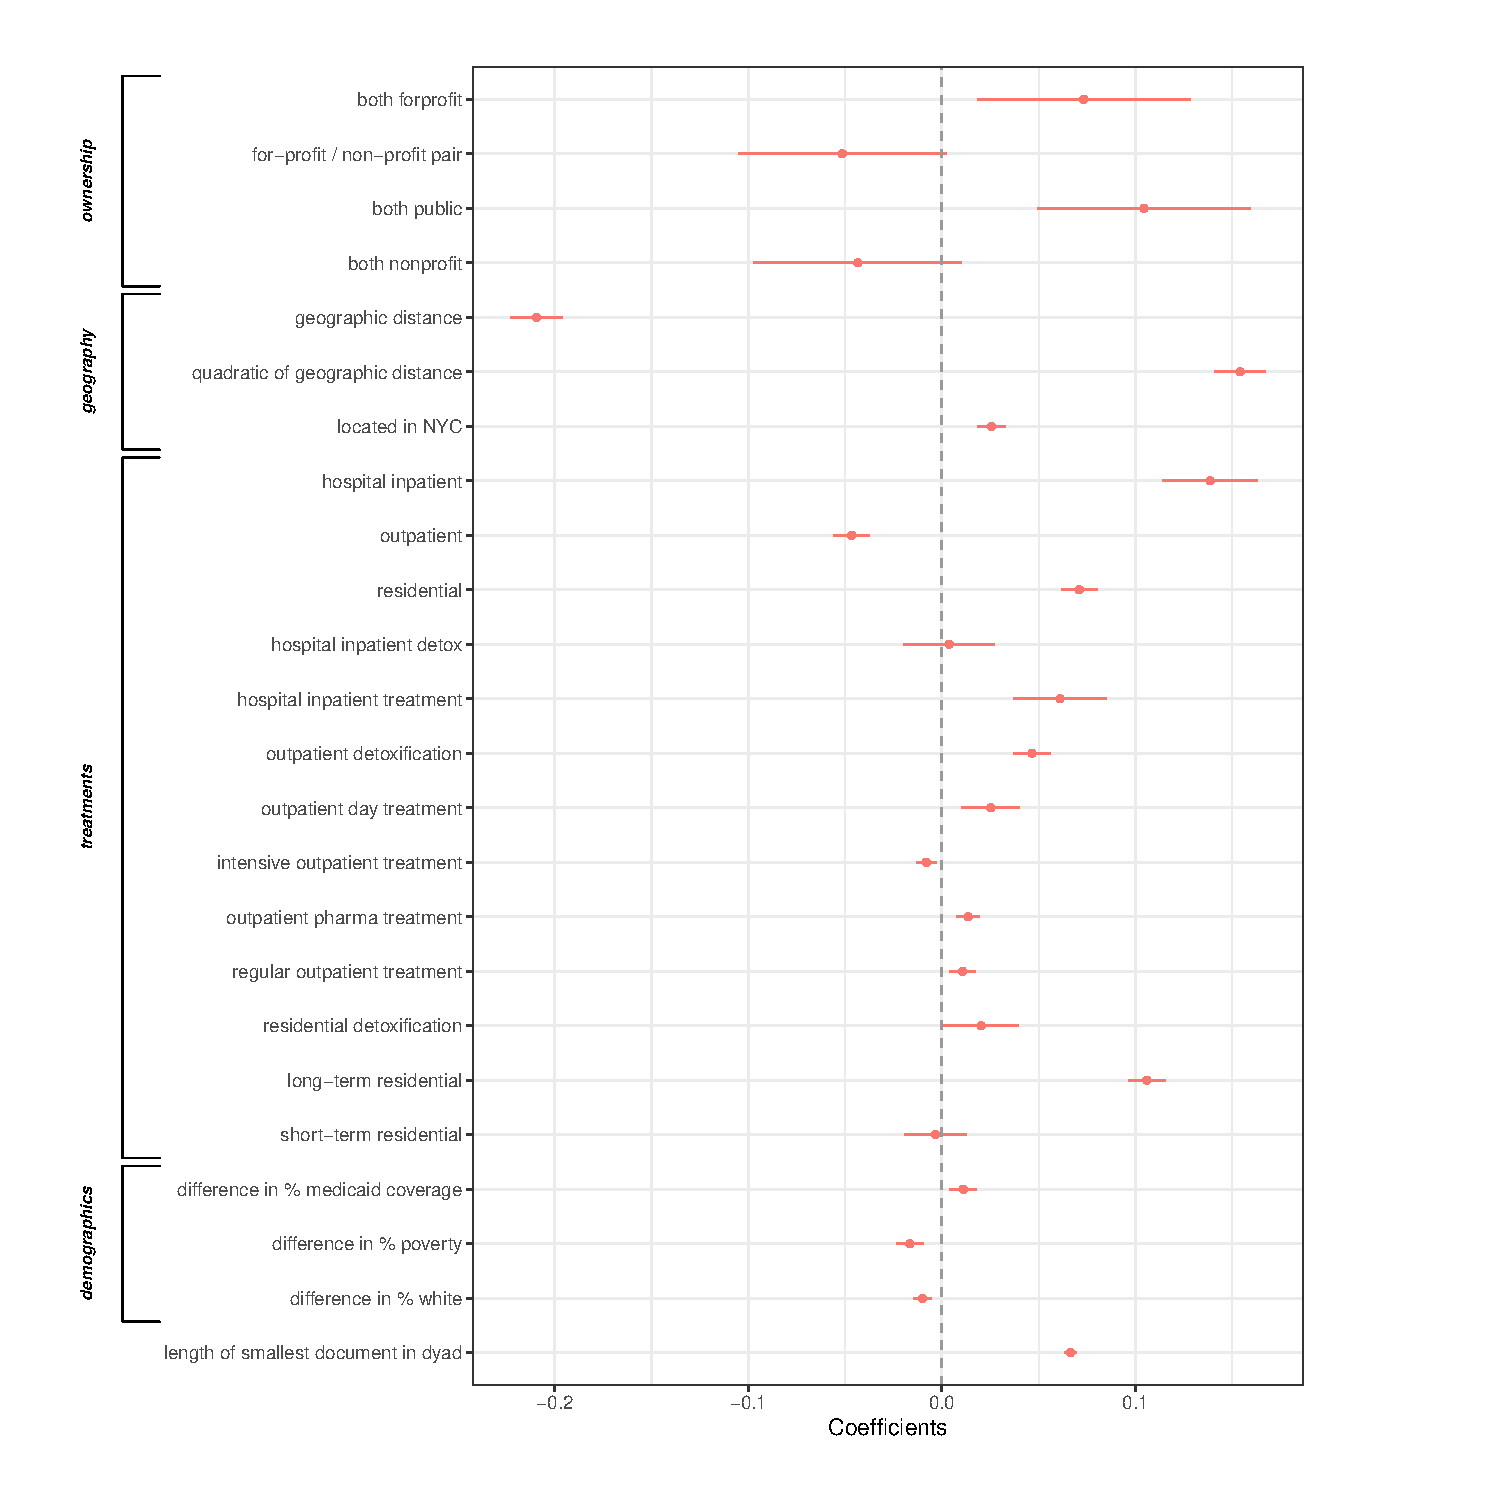
\includegraphics{full_paper_files/figure-latex/unnamed-chunk-5-1} 

}

\caption{\textit{Standardized Mixed-Model Coefficients}}\label{fig:unnamed-chunk-5}
\end{figure}

\vspace{12pt}

In contrast, I find no relationship between sharing non-profit status and semantic similarity. Being non-profit does not seem to affect services' self-presentation. In addition, I find no relationship between non-profit/for-profit pairs and semantic similarity. This rules out the idea that for-profits may imitate their more established non-profit peers.

\vspace{12pt}

I observe these relationships net of other factors that affect semantic similarity. A one standard deviation increase in geographic distance is associated with a 0.2 standard deviation decrease in semantic similarity---as we might expect, the farther apart two services are located from one another, the less likely they are to speak similarly (the quadratic term indicates that this effect becomes more severe as geographic distance increases). In addition, services in New York City tend to speak more similarly to one another. Offering the same treatments tends to have a positive effect on semantic similarity. For example, two services offering long-term residential care speak, on average, 0.1 standard deviations more similarly than services with different treatment offerings\footnote{Interestingly, sharing both outpatient and intensive outpatient treatments is negatively associated with semantic similarity. Future research in the specific character of outpatient treatment is needed to explore this reverse relationship.}.

\vspace{12pt}

Organizations recruit many of their clients from the local areas their services are embedded in. As a result, we might expect local demographic realities to be related to the way organizations present themselves. As expected, I find that the greater the difference in percent poor and percent white between two counties, the less similar the speech of two services embedded within them. Surprisingly, my model suggests that the greater the difference in Medicaid coverage between two counties, the greater the similarity between two services. One possible reason for this surprising finding is that nearly every service accepts Medicaid insurance, so that while the percent of the population eligible might change from county to county, all organizations already present themselves as available to Medicaid patients (although that may not always be their primary audience).

\vspace{12pt}

\hypertarget{exploring-repertoires-of-speech}{%
\subsection{\texorpdfstring{\emph{Exploring repertoires of speech}}{Exploring repertoires of speech}}\label{exploring-repertoires-of-speech}}

Given that, according to my model, for-profit and public services display coherent collective speech, I investigate the context around the keywords ``patient'' and ``client'' and find words most associated with each ownership type. I leave aside non-profits, which did not exhibit coherent collective speech\footnote{Some words do have a higher log-likelihood of being used by non-profits; however, given that my mixed-model finds no evidence of similarity between non-profit services, these words are likely associated with particular non-profit organizations, rather than non-profit services as a whole.}. Table 3 displays the terms most associated with for-profit and public ownership types, as measured by my log-likelihood measure.

\vspace{12pt}

The context around the word \emph{patient} is similarly logistical for both types of ownership---but in two very different sets of ways. For for-profits, words around the keyword \emph{patient} (first column of Table 3) inspire a sense of professionalism and management associated with modern services. References to Suboxone, a contemporary partial agonist medical treatment for opioid addiction, as well as psychotherapy describe what the patient may be receiving from treatment. Terms such as ``disclosure'', ``technique'' and ``authorization'' paint the picture of a well-managed and orchestrated set of services. Other terms specific to for-profit organizations such as ``guarantee'' and ``package'' hint a consolidation of treatment and market logics.

\vspace{12pt}

Words associated with public services and \emph{patient} are similarly logistical. However, the words revealed by my model indicate where the services are located---namely, in larger hospital institutions. References to ``emergency'', ``hospital'', ``unit'' and ``veteran'' draw the patient's attention to the breadth of services that can be accessed in the hospital. A nearly identical type of repertoire is deployed around the word \emph{client}, with some returning words (``lab'', ``video'') and some new terms that evoke that same inclusion in the larger hospital context.

\vspace{12pt}

While the words around both \emph{client} and \emph{patient} did not change much for public organizations, that is not the case of for-profit organizations. Instead, the repertoire utilized by for-profits shift from one keyword to the other. In the case of \emph{client}, we see fewer logistical words and more terms that appeal to reader's emotions such as ``spiritual'', ``emotional'' and ``journey''. For-profits are demonstrating their righteous commitment toward treatment when appealing to individuals as \emph{clients.}

\vspace{12pt}

In sum, my model finds that public organizations define both \emph{patient} and \emph{client} within the context of the hospital institution. Conversely, for-profit organizations leverage several discursive repertoires depending on the keyword being studied. This flexibility in language suggests that the nature of collective speaking is different from public and for-profit organizations. In the case of public organizations, the collective and distinct speech captured by my model may reflect institutional contexts that are intrinsic to public services. On the other hand, for-profits leverage several repertoires strategically, which may put them in a dominant position when defining the discursive parameters of the addiction field.

\begin{table}

\caption{\label{tab:unnamed-chunk-6}Top neighboring words by keyword and ownership}
\centering
\resizebox{\linewidth}{!}{
\begin{tabular}[t]{l|l|l|l}
\hline
\multicolumn{2}{c|}{Patient} & \multicolumn{2}{c}{Client} \\
\cline{1-2} \cline{3-4}
for-profit & public & for-profit & public\\
\hline
suboxone & acute & spiritual & medication\\
\hline
pain & psychiatric & addiction & opioid\\
\hline
physician & emergency & nutritional & receive\\
\hline
alcohol & hospital & pattern & medication\_assisted\_treatment\\
\hline
completely & care & rehab & craving\\
\hline
psychotherapy & unit & account & examination\\
\hline
phase & outreach & addiction\_treatment & lab\\
\hline
explore & video & action & violence\\
\hline
patient & lab & body & domestic\\
\hline
disclosure & adult & emotional & provide\\
\hline
beacon & veteran & inpatient & video\\
\hline
comfortable & clinic & pain & counsel\\
\hline
package & visit & step & service\\
\hline
typical & seek & evaluation & patient\\
\hline
guarantee & mobile & facet & education\\
\hline
behavioral\_health\_services & psychiatry & spirituality & decide\\
\hline
therapeutic & examination & treatment\_plan & doctor\\
\hline
evaluation & competentcentered & clinical & reflective\\
\hline
technique & volunteer & journey & requirement\\
\hline
authorization & service & screen & educational\\
\hline
\end{tabular}}
\end{table}

\hypertarget{discussion}{%
\section{Discussion}\label{discussion}}

The United States finds itself today in the midst of a major transformation in addiction: products abused, where they come from, medications used to treat, and who is treated have all changed significantly in the last few decades. The way addiction, patients, and addiction treatment are spoken about has changed concomitantly. Scholars have extensively documented how language shifts in response to demographic changes in addiction. We know, for example, that the public conversation on addiction changed from the criminal to the medical repertoire as the population of patients became whiter (Taylor et al. \protect\hyperlink{ref-taylor2008}{2008}; Netherland and Hansen \protect\hyperlink{ref-netherland2016}{2016}). Shifts in language also exist in relationship to individual attitudes and behaviors, be it during the construction of patient's family identity (Selbekk and Sagvaag \protect\hyperlink{ref-selbekk2016}{2016}) or struggles for autonomy and privacy (Bourgois \protect\hyperlink{ref-bourgois2000}{2000}). Language both shapes and is shaped by the addiction field.

\vspace{12pt}

The organizational landscape is changing equally rapidly. Increasingly, for-profit ownership is becoming an important feature of the addiction treatment market. Treatment offered by these organizations is often more expensive and of lesser quality; however, their use of specific language gives them an edge in attracting patients (Beetham et al. \protect\hyperlink{ref-beetham2021}{2021}). Despite the importance of language for both organizations and addiction more broadly, we know strikingly little about how ownership relates to the deployment of discourse.

\vspace{12pt}

In this article, I knit together scholarship from new institutionalist theories, the sociology of moral markets and medicalization to determine whether new addiction treatment organizations discursively cohere in the face of heterogenous normative pressure. I suggest two possible mechanisms that may be taking place within the addiction field: a process of isomorphism characterized by a weak relationship between ownership and speech, and a moral market approach characterized by a strong relationship between for-profit ownership and speech. I hypothesize that organizations under the for-profit ownership model face disproportionate normative pressure and would consequently exhibit a strong coherence as expected by moral markets approaches. Using computational social-science methods to determine similarity in speech, I test this hypothesis by studying every addiction treatment service in New York State with an available website. Results demonstrate that for-profit and public organizations produce collective speech; non-profits do not; there is no evidence that for-profits imitate non-profit speech; and for-profits draw on several discursive repertoires. These findings hold even when controlling for other characteristics important to semantic similarity, including geographic distance, treatment offerings and county demographic characteristics.

\vspace{12pt}

In line with the moral markets literature, I find support for my first hypothesis that for-profits exhibit a coherent and multifaceted linguistic approach. My study suggests that for-profit organizations are not engaged in a typical isomorphic process. Faced with normative pressure from within and outside the field, they are not looking to non-profits for linguistic cues. More in line with expectations from the moral markets literature, I find that for-profits are speaking as a collective group distinct from the other two ownership types. My evidence also supports my fourth hypothesis, revealing that for-profit organizations are appealing to readers by meshing language of professionalism and discretion with reference to more emotional aspects of treatment. Not only are for-profit organizations speaking as a coherent group---they are doing so while effectively presenting several repertoires with which prospective readers may resonate (McDonnell, Bail, and Tavory \protect\hyperlink{ref-mcdonnell2017}{2017}).

\vspace{12pt}

Most surprisingly, I do not find evidence of coherent speech among nonprofits. My results do not support my second hypothesis that both public and non-profit ownership would be predictive of semantic similarity, but far less so than for-profit ownership. This may be explained by the particular position held by non-profits in the field of addiction. Non-profit organizations like Phoenix House are hallowed institutions intimately tied to their local area, whose history is archived and remembered (Bertin-Mahieux et al. \protect\hyperlink{ref-bertin-mahieux}{n.d.}). They may be seen as unique organizations, rather than part of a non-profit category. As a result, they are likely to focus their speech on specific treatment and geographic idiosyncrasies rather than looking to one another to cultivate self-presentation.

\vspace{12pt}

On the other hand, public organizations are the most coherent group of the three ownership types compared. One possibility is that public organizations are also under strong normative pressures. Another possibility becomes clear by taking a look at the types of words used to appeal to patients and clients. As evidence for my third hypothesis, I find that public organizations use a single repertoire of language for both patient and client that contrasts with the variety used by for-profit organizations. This repertoire illustrates how public services are embedded in larger hospital institutions. In other words, what is driving similarity between public organizations is language intrinsic to the setting in which public addiction services exist. The signal for collective speech among public organizations is strong---but it may not have the same consequences as collective speech among for-profits.

\vspace{12pt}

These results should give pause to analysts searching for isomorphic processes in collective speech. Ownership types are important predictors of how language clusters---but not equally so. As exemplified in other moralized markets (Livne \protect\hyperlink{ref-livne2014}{2014}), new for-profit entrants have introduced different values to the addiction treatment field. By applying pressure on these organizations to legitimize themselves, conditions were set for for-profits to further solidify their position as offering an alternative to care. In addition, for-profits may not imitate non-profits because there is no coherent model to imitate---only a set of standalone organizations.

\vspace{12pt}

By both producing more coherent language than their non-profit peers and leveraging several alternative repertoires that appeal directly to the reader, for-profit addiction organizations are in a position to negotiate future definitions of addiction. In particular, they have the opportunity to reconcile profit-seeking market values with existing conceptions of addiction care. This consolidation of market and treatment values may have important ramifications for structural inequities and health. This conceptual marriage is likely to yield an increasingly large gap in quality of and access to treatment. Patients who experience domination along class, gender, race and sexuality lines already have worse experiences with addiction treatment (Storbjörk \protect\hyperlink{ref-storbjork2011}{2011}; Saloner and Cook \protect\hyperlink{ref-saloner2013}{2013}). For example, Saloner and Cook (\protect\hyperlink{ref-saloner2013}{2013}) show that black and Hispanic patients are far less likely to complete addiction treatment due to housing instability and providers' lack of cultural competence. This widening gap will only serve to further reinforce these differences. This study thus highlights a particular way in which culture (embodied in collective speech) intersects with social structures to sustain systems of social inequity (Cogburn \protect\hyperlink{ref-cogburn2019}{2019}). The growing field of structural inequality, health and culture has shown how individual behaviors, such as racist internet searches, can have a structural effect on health (Chae et al. \protect\hyperlink{ref-chae2015}{2015}). This study shows the potential for conceiving of culture as emerging among the organizations of a given field.

\vspace{12pt}

Future work should dig deeper into the consequences of collective speech for health outcomes. My current study is limited to New York state, but comparing this relationship across states should yield interesting insight. If cultural forces influence how organizations become central and successful in the market, then we could expect states where non-profit organizations have strong collective messaging to also exhibit fewer inequalities in quality of treatment. In addition, further comparisons beyond the United States could explore how a nation's institutional arrangements and orientation toward addiction treatment marketing influences the quality of care provided. Access to quality healthcare is tied up in market constraints---a better understanding of how these constraints are culturally constructed is a first step toward revealing the power of culture in structuring health outcomes.

\clearpage

\hypertarget{references}{%
\section{References}\label{references}}

\setstretch{1.2}
\setlength{\parindent}{-0.2in}
\setlength{\leftskip}{0.2in}
\setlength{\parskip}{8pt}

\noindent

\hypertarget{refs}{}
\leavevmode\hypertarget{ref-abraham2017}{}%
Abraham, Amanda J., Christina M. Andrews, Colleen M. Grogan, Thomas D'Aunno, Keith N. Humphreys, Harold A. Pollack, and Peter D. Friedmann. 2017. ``The Affordable Care Act Transformation of Substance Use Disorder Treatment.'' \emph{American Journal of Public Health} 107(1):31--32. doi: \href{https://doi.org/10.2105/AJPH.2016.303558}{10.2105/AJPH.2016.303558}.

\leavevmode\hypertarget{ref-acker2002}{}%
Acker, Caroline Jean. 2002. \emph{Creating the American Junkie: Addiction Research in the Classic Era of Narcotic Control}. JHU Press.

\leavevmode\hypertarget{ref-americansocietyofaddictionmedicine2015}{}%
Addiction Medicine, American Society of. 2015. ``The ASAM National Practice Guideline for the Use of Medications in the Treatment of Addiction Involving Opioid Use.''

\leavevmode\hypertarget{ref-nationalassociationofaddictiontreatmentproviders2019}{}%
Addiction Treatment Providers, National Association of. 2019. \emph{Strategic Plan for the Three-Year Period 2019 Through 2021}.

\leavevmode\hypertarget{ref-substanceabuseandmentalhealthservicesadministration2015}{}%
Administration, Substance Abuse and Mental Health Services. 2015. ``Behavioral Health Spending \& Use Accounts 2006---2015.''

\leavevmode\hypertarget{ref-substanceabuseandmentalhealthservicesadministration2020}{}%
Administration, Substance Abuse and Mental Health Services. 2020. ``National Survey of Substance Abuse Treatment Services (N-SSATS): 2019. Data on Substance Abuse Treatment Facilities.''

\leavevmode\hypertarget{ref-andersen2015}{}%
Andersen, Ditte. 2015. ``Stories of Change in Drug Treatment: A Narrative Analysis of `Whats' and `Hows' in Institutional Storytelling.'' \emph{Sociology of Health \& Illness} 37(5):668--82. doi: \href{https://doi.org/10.1111/1467-9566.12228}{10.1111/1467-9566.12228}.

\leavevmode\hypertarget{ref-anteby2010}{}%
Anteby, Michel. 2010. ``Markets, Morals, and Practices of Trade: Jurisdictional Disputes in the U.S. Commerce in Cadavers.'' \emph{Administrative Science Quarterly} 55(4):606--38. doi: \href{https://doi.org/10.2189/asqu.2010.55.4.606}{10.2189/asqu.2010.55.4.606}.

\leavevmode\hypertarget{ref-bachhuber2014}{}%
Bachhuber, Marcus A., William N. Southern, and Chinazo O. Cunningham. 2014. ``Profiting and Providing Less Care: Comprehensive Services at for-Profit, Nonprofit, and Public Opioid Treatment Programs in the United States.'' \emph{Medical Care} 52(5):428--34. doi: \href{https://doi.org/10.1097/MLR.0000000000000121}{10.1097/MLR.0000000000000121}.

\leavevmode\hypertarget{ref-bail2014}{}%
Bail, Christopher A. 2014. ``The Cultural Environment: Measuring Culture with Big Data.'' \emph{Theory and Society} 43(3/4):465--82.

\leavevmode\hypertarget{ref-bail2016}{}%
Bail, Christopher A. 2016. ``Cultural Carrying Capacity: Organ Donation Advocacy, Discursive Framing, and Social Media Engagement.'' \emph{Social Science \& Medicine} 165:280--88. doi: \href{https://doi.org/10.1016/j.socscimed.2016.01.049}{10.1016/j.socscimed.2016.01.049}.

\leavevmode\hypertarget{ref-barry2010}{}%
Barry, Colleen L., Haiden A. Huskamp, and Howard H. Goldman. 2010. ``A Political History of Federal Mental Health and Addiction Insurance Parity.'' \emph{The Milbank Quarterly} 88(3):404--33. doi: \href{https://doi.org/10.1111/j.1468-0009.2010.00605.x}{10.1111/j.1468-0009.2010.00605.x}.

\leavevmode\hypertarget{ref-beetham2021}{}%
Beetham, Tamara, Brendan Saloner, Marema Gaye, Sarah E. Wakeman, Richard G. Frank, and Michael Lawrence Barnett. 2021. ``Admission Practices and Cost of Care for Opioid Use Disorder at Residential Addiction Treatment Programs in the US.'' \emph{Health Affairs} 40(2):317--25. doi: \href{https://doi.org/10.1377/hlthaff.2020.00378}{10.1377/hlthaff.2020.00378}.

\leavevmode\hypertarget{ref-benoit2018}{}%
Benoit, Kenneth, Kohei Watanabe, Haiyan Wang, Paul Nulty, Adam Obeng, Stefan Müller, and Akitaka Matsuo. 2018. ``Quanteda: An R Package for the Quantitative Analysis of Textual Data.'' \emph{Journal of Open Source Software} 3(30):774. doi: \href{https://doi.org/10.21105/joss.00774}{10.21105/joss.00774}.

\leavevmode\hypertarget{ref-bertin-mahieux}{}%
Bertin-Mahieux, Caitlin, Sue Kaplan, Kristin Murphy, Lance Thurner, and Cameron Vanderscoff. n.d. ``Phoenix House Oral History Project.''

\leavevmode\hypertarget{ref-bourgois2000}{}%
Bourgois, P. 2000. ``Disciplining Addictions: The Bio-Politics of Methadone and Heroin in the United States.'' \emph{Culture, Medicine and Psychiatry} 24(2):165--95. doi: \href{https://doi.org/10.1023/a:1005574918294}{10.1023/a:1005574918294}.

\leavevmode\hypertarget{ref-u.scensusbureau2019}{}%
Bureau, U. S. Census. 2019. ``American Community Survey 5-Year Estimates.''

\leavevmode\hypertarget{ref-chae2015}{}%
Chae, David H., Sean Clouston, Mark L. Hatzenbuehler, Michael R. Kramer, Hannah L. F. Cooper, Sacoby M. Wilson, Seth I. Stephens-Davidowitz, Robert S. Gold, and Bruce G. Link. 2015. ``Association Between an Internet-Based Measure of Area Racism and Black Mortality.'' \emph{PLOS ONE} 10(4):e0122963. doi: \href{https://doi.org/10.1371/journal.pone.0122963}{10.1371/journal.pone.0122963}.

\leavevmode\hypertarget{ref-chavez2012}{}%
Chavez, Scott R. 2012. ``Standards for Opioid Treatment in the Criminal Justice System: Implications for Nurses.'' \emph{Journal of Addictions Nursing} 23(1):40--46. doi: \href{https://doi.org/10.3109/10884602.2011.645256}{10.3109/10884602.2011.645256}.

\leavevmode\hypertarget{ref-clarke1992}{}%
Clarke, Lee, and Carroll L. Estes. 1992. ``Sociological and Economic Theories of Markets and Nonprofits: Evidence from Home Health Organizations.'' \emph{American Journal of Sociology} 97(4):945--69.

\leavevmode\hypertarget{ref-cogburn2019}{}%
Cogburn, Courtney D. 2019. ``Culture, Race, and Health: Implications for Racial Inequities and Population Health.'' \emph{The Milbank Quarterly} 97(3):736--61. doi: \href{https://doi.org/10.1111/1468-0009.12411}{10.1111/1468-0009.12411}.

\leavevmode\hypertarget{ref-conrad1992}{}%
Conrad, Peter. 1992. ``Medicalization and Social Control.'' \emph{Annual Review of Sociology} 18:209--32.

\leavevmode\hypertarget{ref-conrad2010}{}%
Conrad, Peter, and Joseph W. Schneider. 2010. \emph{Deviance and Medicalization: From Badness to Sickness}. Temple University Press.

\leavevmode\hypertarget{ref-corredoira2006}{}%
Corredoira, Rafael A., and John R. Kimberly. 2006. ``Industry Evolution Through Consolidation: Implications for Addiction Treatment.'' \emph{Journal of Substance Abuse Treatment} 31(3):255--65. doi: \href{https://doi.org/10.1016/j.jsat.2006.06.020}{10.1016/j.jsat.2006.06.020}.

\leavevmode\hypertarget{ref-dimaggio1990}{}%
DiMaggio, Paul J., and Helmut K. Anheier. 1990. ``The Sociology of Nonprofit Organizations and Sectors.'' \emph{Annual Review of Sociology} 16(1):137--59. doi: \href{https://doi.org/10.1146/annurev.so.16.080190.001033}{10.1146/annurev.so.16.080190.001033}.

\leavevmode\hypertarget{ref-dimaggio1983}{}%
DiMaggio, Paul J., and Walter W. Powell. 1983. ``The Iron Cage Revisited: Institutional Isomorphism and Collective Rationality in Organizational Fields.'' \emph{American Sociological Review} 48(2):147--60. doi: \href{https://doi.org/10.2307/2095101}{10.2307/2095101}.

\leavevmode\hypertarget{ref-centerfordiseasecontrol2020}{}%
Disease Control, Center for. 2020. ``Understanding the Epidemic \textbar{} Drug Overdose \textbar{} CDC Injury Center.'' Retrieved March 17, 2021 (\url{https://www.cdc.gov/drugoverdose/epidemic/index.html}).

\leavevmode\hypertarget{ref-dunning1993}{}%
Dunning, Ted. 1993. ``Accurate Methods for the Statistics of Surprise and Coincidence.'' \emph{Computational Linguistics} 19(1):61--74.

\leavevmode\hypertarget{ref-erreygers2005}{}%
Erreygers, Guido, and Geert Jacobs. 2005. \emph{Language, Communication and the Economy}. John Benjamins Publishing.

\leavevmode\hypertarget{ref-fourcade2007}{}%
Fourcade, Marion, and Kieran Healy. 2007. ``Moral Views of Market Society.'' \emph{Annual Review of Sociology} 33(1):285--311. doi: \href{https://doi.org/10.1146/annurev.soc.33.040406.131642}{10.1146/annurev.soc.33.040406.131642}.

\leavevmode\hypertarget{ref-fuchs2005}{}%
Fuchs, Doris. 2005. ``Commanding Heights? The Strength and Fragility of Business Power in Global Politics.'' \emph{Millennium} 33(3):771--801. doi: \href{https://doi.org/10.1177/03058298050330030501}{10.1177/03058298050330030501}.

\leavevmode\hypertarget{ref-granfield2014}{}%
Granfield, Robert, and Craig Reinarman. 2014. \emph{Expanding Addiction: Critical Essays}. Routledge.

\leavevmode\hypertarget{ref-greenwood2010}{}%
Greenwood, Royston, Amalia Magán Díaz, Stan Xiao Li, and José Céspedes Lorente. 2010. ``The Multiplicity of Institutional Logics and the Heterogeneity of Organizational Responses.'' \emph{Organization Science} 21(2):521--39. doi: \href{https://doi.org/10.1287/orsc.1090.0453}{10.1287/orsc.1090.0453}.

\leavevmode\hypertarget{ref-grogan2020}{}%
Grogan, Colleen M., Clifford S. Bersamira, Phillip M. Singer, Bikki Tran Smith, Harold A. Pollack, Christina M. Andrews, and Amanda J. Abraham. 2020. ``Are Policy Strategies for Addressing the Opioid Epidemic Partisan? A View from the States.'' \emph{Journal of Health Politics, Policy and Law} 45(2):277--309. doi: \href{https://doi.org/10.1215/03616878-8004886}{10.1215/03616878-8004886}.

\leavevmode\hypertarget{ref-guerrero2016}{}%
Guerrero, Erick G., Gregory Aarons, Christine Grella, Bryan R. Garner, Benjamin Cook, and William A. Vega. 2016. ``Program Capacity to Eliminate Outcome Disparities in Addiction Health Services.'' \emph{Administration and Policy in Mental Health} 43(1):23--35. doi: \href{https://doi.org/10.1007/s10488-014-0617-6}{10.1007/s10488-014-0617-6}.

\leavevmode\hypertarget{ref-guerrero2013}{}%
Guerrero, Erick G., and Ahraemi Kim. 2013. ``Organizational Structure, Leadership and Readiness for Change and the Implementation of Organizational Cultural Competence in Addiction Health Services.'' \emph{Evaluation and Program Planning} 40:74--81. doi: \href{https://doi.org/10.1016/j.evalprogplan.2013.05.002}{10.1016/j.evalprogplan.2013.05.002}.

\leavevmode\hypertarget{ref-haber2021}{}%
Haber, Jaren R. 2021. ``Sorting Schools: A Computational Analysis of Charter School Identities and Stratification.'' \emph{Sociology of Education} 94(1):43--64. doi: \href{https://doi.org/10.1177/0038040720953218}{10.1177/0038040720953218}.

\leavevmode\hypertarget{ref-hatcher2018}{}%
Hatcher, Alexandrea E., Sonia Mendoza, and Helena Hansen. 2018. ``At the Expense of a Life: Race, Class, and the Meaning of Buprenorphine in Pharmaceuticalized `Care'.'' \emph{Substance Use \& Misuse} 53(2):301--10.

\leavevmode\hypertarget{ref-healy2010}{}%
Healy, Kieran. 2010. \emph{Last Best Gifts: Altruism and the Market for Human Blood and Organs}. University of Chicago Press.

\leavevmode\hypertarget{ref-henninger2014}{}%
Henninger, Alana, and Hung-En Sung. 2014. ``History of Substance Abuse Treatment.'' Pp. 2257--69 in.

\leavevmode\hypertarget{ref-hughes2008}{}%
Hughes, David, and Peter Vincent-Jones. 2008. ``Schisms in the Church: National Health Service Systems and Institutional Divergence in England and Wales.'' \emph{Journal of Health and Social Behavior} 49(4):400--416. doi: \href{https://doi.org/10.1177/002214650804900403}{10.1177/002214650804900403}.

\leavevmode\hypertarget{ref-iacobucci2018}{}%
Iacobucci, Alaina C., and Emma C. Frieh. 2018. ``(In)Dependence and Addictions: Governmentality Across Public and Private Treatment Discourses.'' \emph{Theoretical Criminology} 22(1):83--98. doi: \href{https://doi.org/10.1177/1362480616667808}{10.1177/1362480616667808}.

\leavevmode\hypertarget{ref-jordan2015}{}%
Jordan, Cassandra. 2015. ``An Alcoholic Forever? A Critical Discourse Analysis of Alcoholics Anonymous Construction of Identity Development in Addiction Recovery.'' M.A., Canada: Royal Roads University (Canada).

\leavevmode\hypertarget{ref-livne2014}{}%
Livne, Roi. 2014. ``Economies of Dying: The Moralization of Economic Scarcity in U.S. Hospice Care.'' \emph{American Sociological Review} 79(5):888--911. doi: \href{https://doi.org/10.1177/0003122414547756}{10.1177/0003122414547756}.

\leavevmode\hypertarget{ref-lounsbury2007}{}%
Lounsbury, Michael. 2007. ``A Tale of Two Cities: Competing Logics and Practice Variation in the Professionalizing of Mutual Funds.'' \emph{The Academy of Management Journal} 50(2):289--307. doi: \href{https://doi.org/10.2307/20159855}{10.2307/20159855}.

\leavevmode\hypertarget{ref-macfarlane2013}{}%
Macfarlane, Fraser, Cathy Barton-Sweeney, Fran Woodard, and Trisha Greenhalgh. 2013. ``Achieving and Sustaining Profound Institutional Change in Healthcare: Case Study Using Neo-Institutional Theory.'' \emph{Social Science \& Medicine} 80:10--18. doi: \href{https://doi.org/10.1016/j.socscimed.2013.01.005}{10.1016/j.socscimed.2013.01.005}.

\leavevmode\hypertarget{ref-maclean2019}{}%
Maclean, Johanna Catherine, and Brendan Saloner. 2019. ``The Effect of Public Insurance Expansions on Substance Use Disorder Treatment: Evidence from the Affordable Care Act.'' \emph{Journal of Policy Analysis and Management : {[}The Journal of the Association for Public Policy Analysis and Management{]}} 38(2):366--93.

\leavevmode\hypertarget{ref-mann2021}{}%
Mann. 2021. ``As Addiction Deaths Surge, Profit-Driven Rehab Industry Faces 'Severe Ethical Crisis'.'' \emph{NPR.org}.

\leavevmode\hypertarget{ref-mcdonnell2017}{}%
McDonnell, Terence E., Christopher A. Bail, and Iddo Tavory. 2017. ``A Theory of Resonance.'' \emph{Sociological Theory} 35(1):1--14. doi: \href{https://doi.org/10.1177/0735275117692837}{10.1177/0735275117692837}.

\leavevmode\hypertarget{ref-meyer2018}{}%
Meyer. 2018. ``Investors Pour Money into Addiction Treatment, but Quality Questions Remain.'' \emph{Modern Healthcare: Providers}, November 24.

\leavevmode\hypertarget{ref-mohr1994}{}%
Mohr, John W. 1994. ``Soldiers, Mothers, Tramps and Others: Discourse Roles in the 1907 New York City Charity Directory.'' \emph{Poetics} 22(4):327--57. doi: \href{https://doi.org/10.1016/0304-422X(94)90013-2}{10.1016/0304-422X(94)90013-2}.

\leavevmode\hypertarget{ref-mohr1997}{}%
Mohr, John W., and Vincent Duquenne. 1997. ``The Duality of Culture and Practice: Poverty Relief in New York City, 1888-1917.'' \emph{Theory and Society} 26(2/3):305--56.

\leavevmode\hypertarget{ref-nelson2017}{}%
Nelson, Laura K. 2017. ``Computational Grounded Theory: A Methodological Framework.'' \emph{Sociological Methods \& Research} 0049124117729703. doi: \href{https://doi.org/10.1177/0049124117729703}{10.1177/0049124117729703}.

\leavevmode\hypertarget{ref-netherland2016}{}%
Netherland, Julie, and Helena B. Hansen. 2016. ``The War on Drugs That Wasn't: Wasted Whiteness, "Dirty Doctors," and Race in Media Coverage of Prescription Opioid Misuse.'' \emph{Culture, Medicine and Psychiatry; New York} 40(4):664--86. doi: \href{https://doi.org/http://dx.doi.org.proxy.lib.duke.edu/10.1007/s11013-016-9496-5}{http://dx.doi.org.proxy.lib.duke.edu/10.1007/s11013-016-9496-5}.

\leavevmode\hypertarget{ref-parsons1951}{}%
Parsons, Talcott, 1902-1979. 1951. \emph{The Social System.} New York: New York, Free Press ; London, Collier-Macmillan {[}1964, c1951{]}.

\leavevmode\hypertarget{ref-paxton2020}{}%
Paxton, Pamela, Kristopher Velasco, and Robert W. Ressler. 2020. ``Does Use of Emotion Increase Donations and Volunteers for Nonprofits?'' \emph{American Sociological Review} 85(6):1051--83. doi: \href{https://doi.org/10.1177/0003122420960104}{10.1177/0003122420960104}.

\leavevmode\hypertarget{ref-reich2014}{}%
Reich, Adam D. 2014. ``Contradictions in the Commodification of Hospital Care.'' \emph{American Journal of Sociology} 119(6):1576--1628. doi: \href{https://doi.org/10.1086/676836}{10.1086/676836}.

\leavevmode\hypertarget{ref-riboni2020}{}%
Riboni, Giorgia. 2020. ``Representation of Knowledge About Opioid Addiction Between Criminalization and Medicalization.'' \emph{Anglistica AION} 23(1):123--39. doi: \href{https://doi.org/10.19231/angl-aion.201918}{10.19231/angl-aion.201918}.

\leavevmode\hypertarget{ref-rudd2014}{}%
Rudd. 2014. ``Increases in Heroin Overdose Deaths --- 28 States, 2010 to 2012.'' Retrieved March 17, 2021 (\url{https://www.cdc.gov/mmwr/preview/mmwrhtml/mm6339a1.htm}).

\leavevmode\hypertarget{ref-saloner2013}{}%
Saloner, Brendan, and Benjamin Lê Cook. 2013. ``Blacks and Hispanics Are Less Likely Than Whites to Complete Addiction Treatment, Largely Due to Socioeconomic Factors.'' \emph{H E a Lt H A F Fai R S} 11.

\leavevmode\hypertarget{ref-scott2000}{}%
Scott, W. Richard, Martin Ruef, Martin (University of North Carolina Ruef USA), Peter J. Mendel, and Carol A. Caronna. 2000. \emph{Institutional Change and Healthcare Organizations: From Professional Dominance to Managed Care}. University of Chicago Press.

\leavevmode\hypertarget{ref-segal2017}{}%
Segal, David. 2017. ``In Pursuit of Liquid Gold.'' \emph{The New York Times: Business}, December 27.

\leavevmode\hypertarget{ref-selbekk2016}{}%
Selbekk, Anne Schanche, and Hildegunn Sagvaag. 2016. ``Troubled Families and Individualised Solutions: An Institutional Discourse Analysis of Alcohol and Drug Treatment Practices Involving Affected Others.'' \emph{Sociology of Health \& Illness} 38(7):1058--73. doi: \href{https://doi.org/10.1111/1467-9566.12432}{10.1111/1467-9566.12432}.

\leavevmode\hypertarget{ref-simpson2007}{}%
Simpson, D. Dwayne, George W. Joe, and Grace A. Rowan-Szal. 2007. ``Linking the Elements of Change: Program and Client Responses to Innovation.'' \emph{Journal of Substance Abuse Treatment} 33(2):201--9. doi: \href{https://doi.org/10.1016/j.jsat.2006.12.022}{10.1016/j.jsat.2006.12.022}.

\leavevmode\hypertarget{ref-sitikhu2019}{}%
Sitikhu, Pinky, Kritish Pahi, Pujan Thapa, and Subarna Shakya. 2019. ``A Comparison of Semantic Similarity Methods for Maximum Human Interpretability.'' Retrieved March 29, 2021 (\url{http://arxiv.org/abs/1910.09129}).

\leavevmode\hypertarget{ref-sparckjones1972}{}%
Sparck Jones, Karen. 1972. ``A Statistical Interpretation of Term Specificity and Its Application in Retrieval.'' \emph{Journal of Documentation} 28(1):11--21. doi: \href{https://doi.org/10.1108/eb026526}{10.1108/eb026526}.

\leavevmode\hypertarget{ref-staton2021}{}%
Staton, Monte D., Barbara Andraka-Christou, and Dennis P. Watson. 2021. ``Isomorphic Pressures on Jail Diversion: From Serious Mental Illness to Opioid Use Disorder.'' \emph{The Prison Journal} 101(2):187--209. doi: \href{https://doi.org/10.1177/0032885521991092}{10.1177/0032885521991092}.

\leavevmode\hypertarget{ref-stinchcombe2000}{}%
Stinchcombe, Arthur L. 2000. ``Social Structure and Organizations.'' Pp. 229--59 in \emph{Economics Meets Sociology in Strategic Management}. Vol. 17, \emph{Advances in Strategic Management}, edited by J. A. C. Baum and F. Dobbin. Emerald Group Publishing Limited.

\leavevmode\hypertarget{ref-storbjork2011}{}%
Storbjörk, Jessica. 2011. ``Gender Differences in Substance Use, Problems, Social Situation and Treatment Experiences Among Clients Entering Addiction Treatment in Stockholm.'' \emph{Nordic Studies on Alcohol and Drugs} 28(3):185--209. doi: \href{https://doi.org/10.2478/v10199-011-0020-5}{10.2478/v10199-011-0020-5}.

\leavevmode\hypertarget{ref-storbjork2019}{}%
Storbjörk, Jessica, and Kerstin Stenius. 2019. ``Why Research Should Pay Attention to Effects of Marketization of Addiction Treatment Systems.'' \emph{Journal of Studies on Alcohol and Drugs, Supplement} (s18):31--39. doi: \href{https://doi.org/10.15288/jsads.2019.s18.31}{10.15288/jsads.2019.s18.31}.

\leavevmode\hypertarget{ref-taylor2008}{}%
Taylor, Copyright, Francis Group, Matthew L. Newman, Carla J. Groom, Lori D. Handelman, and James W. Pennebaker. 2008. \emph{Gender Differences in Language Use: An Analysis of 14,000 Text Samples}.

\leavevmode\hypertarget{ref-turco2012}{}%
Turco, Catherine. 2012. ``Difficult Decoupling: Employee Resistance to the Commercialization of Personal Settings.'' \emph{American Journal of Sociology} 118(2):380--419. doi: \href{https://doi.org/10.1086/666505}{10.1086/666505}.

\leavevmode\hypertarget{ref-weber2011}{}%
Weber, Klaus, and M. Tina Dacin. 2011. ``The Cultural Construction of Organizational Life: Introduction to the Special Issue.'' \emph{Organization Science} 22(2):287--98. doi: \href{https://doi.org/10.1287/orsc.1100.0632}{10.1287/orsc.1100.0632}.

\leavevmode\hypertarget{ref-wetts2020}{}%
Wetts, Rachel. 2020. ``Models and Morals: Elite-Oriented and Value-Neutral Discourse Dominates American Organizations' Framings of Climate Change.'' \emph{Social Forces} 98(3):1339--69. doi: \href{https://doi.org/10.1093/sf/soz027}{10.1093/sf/soz027}.

\leavevmode\hypertarget{ref-you2016}{}%
You, Kai, Yue Li, Orna Intrator, David Stevenson, Richard Hirth, David Grabowski, and Jane Banaszak-Holl. 2016. ``Do Nursing Home Chain Size and Proprietary Status Affect Experiences with Care?'' \emph{Medical Care} 54(3):229--34. doi: \href{https://doi.org/10.1097/MLR.0000000000000479}{10.1097/MLR.0000000000000479}.

\leavevmode\hypertarget{ref-zhao2021}{}%
Zhao, Xinyan, and Hyun Jee Oh. 2021. ``What Fosters Interorganizational Frame Convergence: Examining a Semantic Network During the Opioid Crisis.'' \emph{Public Relations Review} 47(3):102042. doi: \href{https://doi.org/10.1016/j.pubrev.2021.102042}{10.1016/j.pubrev.2021.102042}.

\clearpage

\appendix
\addtocontents{toc}{\protect\setcounter{tocdepth}{2}}

\renewcommand{\thesection}{A}

\setcounter{page}{1}

\setcounter{table}{0}
\renewcommand{\thetable}{A\arabic{table}}
\renewcommand{\figurename}{Table}

\setcounter{figure}{0}
\renewcommand\thefigure{A\arabic{figure}}
\renewcommand{\figurename}{Figure}

\clearpage
\pagenumbering{gobble}

\vspace*{7cm}

\begin{center}
\begin{huge}
Appendix A: Full mixed-effects models with additive terms
\end{huge}
\end{center}
\vspace{3cm}

\clearpage
\pagenumbering{arabic}

\begin{table}[!htbp] \centering 
  \caption{Mixed Models} 
  \label{} 
\tiny 
\begin{tabular}{@{\extracolsep{0pt}}lccccc} 
\\[-1.8ex]\hline 
\hline \\[-1.8ex] 
 & \multicolumn{5}{c}{\textit{Dependent variable:}} \\ 
\cline{2-6} 
\\[-1.8ex] & \multicolumn{5}{c}{Semantic Similarity} \\ 
\\[-1.8ex] & (1) & (2) & (3) & (4) & (5)\\ 
\hline \\[-1.8ex] 
 Both for-profit & 0.082$^{***}$ & 0.076$^{***}$ & 0.075$^{***}$ & 0.073$^{***}$ & 0.073$^{***}$ \\ 
  & (0.028) & (0.028) & (0.028) & (0.028) & (0.028) \\ 
  & & & & & \\ 
 For-profit/Non-profit pair & $-$0.048$^{*}$ & $-$0.050$^{*}$ & $-$0.051$^{*}$ & $-$0.052$^{*}$ & $-$0.051$^{*}$ \\ 
  & (0.027) & (0.027) & (0.028) & (0.028) & (0.027) \\ 
  & & & & & \\ 
 Both public & 0.096$^{***}$ & 0.100$^{***}$ & 0.101$^{***}$ & 0.104$^{***}$ & 0.104$^{***}$ \\ 
  & (0.028) & (0.028) & (0.028) & (0.028) & (0.028) \\ 
  & & & & & \\ 
 Both non-profit & $-$0.038 & $-$0.040 & $-$0.040 & $-$0.043 & $-$0.043 \\ 
  & (0.027) & (0.027) & (0.027) & (0.027) & (0.027) \\ 
  & & & & & \\ 
 Geographic distance &  & $-$0.262$^{***}$ & $-$0.219$^{***}$ & $-$0.217$^{***}$ & $-$0.209$^{***}$ \\ 
  &  & (0.006) & (0.007) & (0.007) & (0.007) \\ 
  & & & & & \\ 
 Quadratic of geographic distance &  & 0.197$^{***}$ & 0.161$^{***}$ & 0.161$^{***}$ & 0.154$^{***}$ \\ 
  &  & (0.006) & (0.007) & (0.007) & (0.007) \\ 
  & & & & & \\ 
 New York City &  &  & 0.040$^{***}$ & 0.040$^{***}$ & 0.026$^{***}$ \\ 
  &  &  & (0.003) & (0.003) & (0.004) \\ 
  & & & & & \\ 
 Hospital inpatient &  &  &  & 0.139$^{***}$ & 0.139$^{***}$ \\ 
  &  &  &  & (0.012) & (0.012) \\ 
  & & & & & \\ 
 Outpatient &  &  &  & $-$0.046$^{***}$ & $-$0.047$^{***}$ \\ 
  &  &  &  & (0.005) & (0.005) \\ 
  & & & & & \\ 
 Residential &  &  &  & 0.071$^{***}$ & 0.071$^{***}$ \\ 
  &  &  &  & (0.005) & (0.005) \\ 
  & & & & & \\ 
 Hospital inpatient detox &  &  &  & 0.004 & 0.004 \\ 
  &  &  &  & (0.012) & (0.012) \\ 
  & & & & & \\ 
 Hospital inpatient treatment &  &  &  & 0.061$^{***}$ & 0.061$^{***}$ \\ 
  &  &  &  & (0.012) & (0.012) \\ 
  & & & & & \\ 
 Outpatient detox &  &  &  & 0.046$^{***}$ & 0.047$^{***}$ \\ 
  &  &  &  & (0.005) & (0.005) \\ 
  & & & & & \\ 
 Outpatient day treatment &  &  &  & 0.026$^{***}$ & 0.025$^{***}$ \\ 
  &  &  &  & (0.008) & (0.008) \\ 
  & & & & & \\ 
 Intensive outpatient treatment &  &  &  & $-$0.008$^{***}$ & $-$0.008$^{***}$ \\ 
  &  &  &  & (0.003) & (0.003) \\ 
  & & & & & \\ 
 Outpatient pharmaceutical treatment &  &  &  & 0.013$^{***}$ & 0.014$^{***}$ \\ 
  &  &  &  & (0.003) & (0.003) \\ 
  & & & & & \\ 
 Regular outpatient treatment &  &  &  & 0.011$^{***}$ & 0.011$^{***}$ \\ 
  &  &  &  & (0.003) & (0.003) \\ 
  & & & & & \\ 
 Residential detox &  &  &  & 0.020$^{**}$ & 0.020$^{**}$ \\ 
  &  &  &  & (0.010) & (0.010) \\ 
  & & & & & \\ 
 Long-term residential &  &  &  & 0.106$^{***}$ & 0.106$^{***}$ \\ 
  &  &  &  & (0.005) & (0.005) \\ 
  & & & & & \\ 
 Short-term residential &  &  &  & $-$0.003 & $-$0.003 \\ 
  &  &  &  & (0.008) & (0.008) \\ 
  & & & & & \\ 
 Difference in pct medicaid coverage &  &  &  &  & 0.011$^{***}$ \\ 
  &  &  &  &  & (0.004) \\ 
  & & & & & \\ 
 Difference in pct poverty &  &  &  &  & $-$0.016$^{***}$ \\ 
  &  &  &  &  & (0.004) \\ 
  & & & & & \\ 
 Difference in pct white &  &  &  &  & $-$0.010$^{***}$ \\ 
  &  &  &  &  & (0.002) \\ 
  & & & & & \\ 
 Length of smallest document in pair & 0.072$^{***}$ & 0.072$^{***}$ & 0.072$^{***}$ & 0.067$^{***}$ & 0.067$^{***}$ \\ 
  & (0.002) & (0.002) & (0.002) & (0.002) & (0.002) \\ 
  & & & & & \\ 
 Constant & 0.152$^{***}$ & 0.147$^{***}$ & 0.177$^{***}$ & 0.622$^{***}$ & 0.611$^{***}$ \\ 
  & (0.034) & (0.034) & (0.034) & (0.039) & (0.039) \\ 
  & & & & & \\ 
\hline \\[-1.8ex] 
Observations & 271,672 & 271,672 & 271,672 & 271,672 & 271,672 \\ 
Log Likelihood & $-$219,154.600 & $-$217,114.600 & $-$217,010.600 & $-$215,332.600 & $-$215,326.100 \\ 
Akaike Inf. Crit. & 438,327.100 & 434,251.200 & 434,045.100 & 430,715.200 & 430,708.200 \\ 
Bayesian Inf. Crit. & 438,421.800 & 434,366.800 & 434,171.300 & 430,978.000 & 431,002.500 \\ 
\hline 
\hline \\[-1.8ex] 
\textit{Note:}  & \multicolumn{5}{r}{$^{*}$p$<$0.1; $^{**}$p$<$0.05; $^{***}$p$<$0.01} \\ 
\end{tabular} 
\end{table}

\clearpage

\vspace*{7cm}

\begin{center}
\begin{huge}
Appendix B: Model fit for tested models
\end{huge}
\end{center}
\vspace{3cm}

\clearpage

\renewcommand{\arraystretch}{2}

\begin{table}

\caption{\label{tab:unnamed-chunk-7}Fitting models and associated BIC values}
\centering
\resizebox{\linewidth}{!}{
\begin{tabular}[t]{l|r}
\hline
model terms & BIC values\\
\hline
ownership homophily + treatment/geographic controls + ACS + non-profit/for-profit + NYC & 431002.5\\
\hline
ownership homophily + treatment/geographic controls + ACS & 431016.8\\
\hline
ownership homophily + treatment/geographic controls + non-profit/for-profit & 431031.2\\
\hline
ownership homophily*geography + non-profit/for-profit*geography + treatment controls + NYC + ACS & 431039.6\\
\hline
ownership homophily*ACS + treatment/geographic controls + non-profit/for-profit + NYC & 431069.4\\
\hline
ownership homophily*ACS + treatment/geographic controls & 431083.8\\
\hline
ownership homophily*ACS + non-profit/for-profit*ACS + treatment/geographic controls & 431125.2\\
\hline
ownership homophily + treatment/geographic controls & 431166.8\\
\hline
ownership homophily & 434801.8\\
\hline
\end{tabular}}
\end{table}

\end{document}
